\documentclass[12pt]{article}
\usepackage{graphicx,import}
\usepackage[svgnames]{xcolor} 
\usepackage{fancyhdr}
\usepackage{subfig}
\usepackage{hyperref}
\usepackage{enumitem}
\usepackage{cite}
\usepackage[many]{tcolorbox}
\usepackage{listings }
\usepackage[a4paper, total={6in, 8in} , bottom = 25mm , top = 25mm, headheight = 1.25cm , includehead,includefoot,heightrounded ]{geometry}
\usepackage{afterpage}
\usepackage{amssymb}
\usepackage{pdflscape}
\usepackage{textcomp}
\usepackage{xecolor}
\usepackage{rotating}
\usepackage{pdfpages}
\usepackage[Kashida]{xepersian}
\usepackage[T1]{fontenc}
\usepackage{tikz}
\usepackage[utf8]{inputenc}
\usepackage{PTSerif} 
\usepackage{seqsplit}

\usepackage[edges]{forest}

\usepackage{listings}
\usepackage{xcolor}

\hypersetup{
	colorlinks   = true, %Colours links instead of ugly boxes
	urlcolor     = blue, %Colour for external hyperlinks
	linkcolor    = blue, %Colour of internal links
	citecolor   = red %Colour of citations
}
 
\definecolor{codegreen}{rgb}{0,0.6,0}
\definecolor{codegray}{rgb}{0.5,0.5,0.5}
\definecolor{codepurple}{rgb}{0.58,0,0.82}
\definecolor{backcolour}{rgb}{0.95,0.95,0.92}
 
\NewDocumentCommand{\codeword}{v}{
\texttt{\textcolor{blue}{#1}}
}
\lstset{language=java,keywordstyle={\bfseries \color{blue}}}

\lstdefinestyle{mystyle}{
    backgroundcolor=\color{backcolour},   
    commentstyle=\color{codegreen},
    keywordstyle=\color{magenta},
    numberstyle=\tiny\color{codegray},
    stringstyle=\color{codepurple},
    basicstyle=\ttfamily\normalsize,
    breakatwhitespace=false,         
    breaklines=true,                 
    captionpos=b,                    
    keepspaces=true,                 
    numbers=left,                    
    numbersep=5pt,                  
    showspaces=false,                
    showstringspaces=false,
    showtabs=false,                  
    tabsize=2
}

\lstset{style=mystyle}

\settextfont[Scale=1.2 ,BoldFont={Bahij Nazanin-Bold.ttf} , ItalicFont = {IRNazaninIranic.ttf}]{Bahij Nazanin-Regular.ttf}
\DefaultMathsDigits 
\DeclareMathSizes{11}{19}{13}{9} 
%\DeclareMathSizes{12}{14.4}{8}{9}





\newenvironment{changemargin}[2]{%
\begin{list}{}{%
\setlength{\topsep}{0pt}%
\setlength{\leftmargin}{#1}%
\setlength{\rightmargin}{#2}%
\setlength{\listparindent}{\parindent}%
\setlength{\itemindent}{\parindent}%
\setlength{\parsep}{\parskip}%
}%
\item[]}{\end{list}}


\definecolor{foldercolor}{RGB}{124,166,198}

\tikzset{pics/folder/.style={code={%
    \node[inner sep=0pt, minimum size=#1](-foldericon){};
    \node[folder style, inner sep=0pt, minimum width=0.3*#1, minimum height=0.6*#1, above right, xshift=0.05*#1] at (-foldericon.west){};
    \node[folder style, inner sep=0pt, minimum size=#1] at (-foldericon.center){};}
    },
    pics/folder/.default={20pt},
    folder style/.style={draw=foldercolor!80!black,top color=foldercolor!40,bottom color=foldercolor}
}

\forestset{is file/.style={edge path'/.expanded={%
        ([xshift=\forestregister{folder indent}]!u.parent anchor) |- (.child anchor)},
        inner sep=1pt},
    this folder size/.style={edge path'/.expanded={%
        ([xshift=\forestregister{folder indent}]!u.parent anchor) |- (.child anchor) pic[solid]{folder=#1}}, inner xsep=0.6*#1},
    folder tree indent/.style={before computing xy={l=#1}},
    folder icons/.style={folder, this folder size=#1, folder tree indent=3*#1},
    folder icons/.default={12pt},
}

\begin{document}


%%% title pages
\begin{titlepage}
\begin{center}
        
\vspace*{0.7cm}

\vspace{0.5cm}
\textbf{ \Huge{\emph ‌مقدمه‌ای بر بیوانفورماتیک} }\\
\vspace{0.5cm}
\textbf{ \Large{ پروژه پایانی} }
\vspace{0.2cm}
       
 
      \large \textbf{دانشکده مهندسی کامپیوتر}\\\vspace{0.2cm}
    \large   دانشگاه صنعتی شریف\\\vspace{0.2cm}
       \large   ﻧﯿﻢ سال اول 01-00 \\\vspace{0.2cm}
      \noindent\rule[1ex]{\linewidth}{1pt}
اساتید:\\
 \vspace{0.30cm}
    \textbf{{جناب آقای دکتر شریفی و سرکار خانم دکتر کوﮬـی}}


    \vspace{0.40cm}
نام و نام خانوادگی:\\

        \vspace{0.30cm}
    \textbf{{
ایمان علیپور
    }}
    
        \vspace{0.40cm}
شماره دانشجویی:\\

        \vspace{0.30cm}
    \textbf{{
98102024
    }}
\end{center}
\end{titlepage}
%%% title pages


%%% header of pages
\newpage
\pagestyle{fancy}
\fancyhf{}
\fancyfoot{}
\cfoot{\thepage}
\chead{پروژه نهایی مقدمه‌ای بر بیوانفورماتیک}
\lhead{
ایمان علیپور
}
%%% header of pages

\KashidaOff


\section{مقدمه}

در این پروژه، قصد داریم به تحلیل داده‌های ریزآرایه
\LTRfootnote{Microarray}
 برای لوکمی حاد مغزاستخوان
\LTRfootnote{Acute myeloid leukemia (AML) }
بپردازیم. این بیماری نوعی سرطان خون و مغز استخوان است که در آن سلول‌های میلوئیدی
 \LTRfootnote{Myeloid}
 مغز استخوان، به تعداد بیش‌تری تکثیر می‌شوند. این موضوع منجر به تولید بیش‌از اندازه پیش‌سازهای گلبول‌های سفید 
\LTRfootnote{Precursor Blood Cells}
 می‌شود اما این پیش‌سازها توانایی مقابله با عفونت‌ها را ندارند و در نتیجه بدن نسبت به عفونت ضعیف می‌شود. در این بیماری شاهد نوعی از کم‌خونی و کاهش تعداد گلبول‌های قرمز اصلی بدن می‌شود و در عوض سلول‌های خونی غیرعادی تولید می‌شود که منجر به نارسایی‌های مختلف در فرد بیمار می‌شود.
 
 در این پروژه به کمک داده‌های ریزآرایه قصد داریم ارتباط بین تغییرات بیان‌ژن در افراد مبتلا به این بیماری را مشخص کنیم و سپس براساس ژن‌هایی که تغییر بیان را نشان می‌دهند، در مورد مسیر های زیستی
 \LTRfootnote{Pathway}
مرتبط با این ژن‌ها
  \LTRfootnote{Gene} 
 و عملکرد آنان، اطلاعاتی را ارائه کنیم.
 
\section{آماده سازی اولیه}

در ابتدای کد تمامی کتابخانه‌های مورد نیاز را اضافه می‌کنیم:

\begin{latin}
\begin{lstlisting}[language=R]
	library(GEOquery)
	library(limma)
	library(Biobase)
	library(pheatmap)
	library(reshape2)
	library(plyr)
	library(ggplot2)
	library(stringr)
	library(gplots)
\end{lstlisting}
\end{latin}
توجه کنید که من در نوشتن کدهای این پروژه، از ویدیوهای دکتر شریفی زارچی واقع در این 
\href{https://maktabkhooneh.org/course/%D8%A8%DB%8C%D9%88%D8%A7%D9%86%D9%81%D9%88%D8%B1%D9%85%D8%A7%D8%AA%DB%8C%DA%A9-%D9%BE%DB%8C%D8%B4%D8%B1%D9%81%D8%AA%D9%87-mk375/}{لینک} 
استفاده کردم و شباهت بسیار زیادی بین این کدها و کدهای دکتر شریفی وجود دارد، همچنین در فایل \lr{Analysis.R} که به همراه این مستند تحویل داده شده است، برای همه تکه های مختلف کد کامنت گذاری کردم تا دقیقا مشخص باشد دارم چه کاری انجام میدهم.

بعد از اضافه کردن کتابخانه های مورد نیاز، باید داده‌ها را به کمک کتابخانه \lr{GEOquery} بخوانیم. با توجه به لینک داده شده در مستند تعریف پروژه،  متوجه می‌شویم که نام دیتاست مورد استفاده \lr{GSE48558} و بر پایه پلتفرم \lr{GPL6244} است. این دو عبارت را به صورت یک متغیر ذخیره می‌کنیم تا اگر بعدها خواستیم تحلیل را روی دیتاست مشابهی انجام دهیم، این قسمت کد بدون تغییر قابل استفاده باشد.

\begin{latin}
	\begin{lstlisting}[language=R]
		gset <- getGEO(series_name, GSEMatrix =TRUE, AnnotGPL=TRUE , destdir = "Data")
		if (length(gset) > 1){
			idx <- grep(platform_name, attr(gset, "names"))
		} else {
			idx <- 1
		}
		gset <- gset[[idx]]
	\end{lstlisting}
\end{latin}


عبارت \lr{if} گذاشته شده برای این است که اگر دیتاست روی چند پلتفرم مختلف موجود باشد، دیتای یکی از آن‌ها را انتخاب کنیم. در این جا البته این طور نیست و در اصل همان حالت \lr{else} اتفاق می افتد،
خود دکتر شریفی هم با چک کردن تعداد پلتفرم ها و دادن ایندکس دستی این کار را انجام دادند، ما هم میتوانستیم کار مشابهی انجام دهیم.


حال نوبت به انتخاب و اسم گذاری روی گروه‌ها می‌رسد. برای این کار مواردی که مربوط به بیماری بودند، همگی \lr{Test} نامگذاری شده‌اند. برای مواردی که \lr{Normal} بودند، نوع Source Name هم به انتها نام گروه آن‌ها اضافه شده است چون در ادامه کار برای انجام تحلیل‌ها به آن‌ها نیاز داریم. ضمناً اینکه برای \lr{CD34ُ}، کلمه اضافی \lr{HSPC} هم وجود داشت که از نام گروه خارج شده است.

\begin{latin}
	\begin{lstlisting}[language=R]
		gset<- gset[,which(gset$source_name_ch1 == "AML Patient" | gset$`phenotype:ch1` == "Normal")]
		func <- function(x) {
			if (gset$source_name_ch1[x] == "AML Patient") {
				return("Test")
			} else {
				spll <- strsplit2(gset$source_name_ch1[x] , "\\+")[1, 1]
				return(paste0("Normal_" , spll))
			}
		}
		
		
		
		gr <- sapply(1:length(gset$`phenotype:ch1`) , func)
\end{lstlisting}
\end{latin}

 
 
\section{نرمال سازی داده ها}

ابتدا ماتریس بیان ژن را تشکیل می‌دهیم و ماکسیمم و مینیمم آن را چک می‌کنیم.



\begin{latin}
	\begin{lstlisting}[language=R]
	expr <- exprs(gset)
	print(paste0("Max Expr: " , max(expr)))
	print(paste0("Min Expr: " , min(expr)))
	\end{lstlisting}
\end{latin}

خروجی این دو پرینت قسمت عبارات زیر است:
\begin{latin}
\begin{verbatim}
	"Max Expr: 13.76153622"
	"Min Expr: 1.611473179"
\end{verbatim}
\end{latin}


این نشان دهنده این است که داده ها در \textbf{مقیاس لگاریتمی هستند و نیازی به تغییر مقیاس نداریم.}
دلیل این حرف هم این است که مقدار ماکسیمم عدد کوچکی اتس، اگر این مقدار مثلا پنج‌هزار بود، میتوانستیم بگوییم داده‌ها در مقیاس لگاریتمی نیستند و باید تبدیل شوند، همچنین
کد تبدیل کننده به مقیاس لگاریتمی هم در فایل اصلی به صورت کامنت شده موجود است.

\subsection{بررسی نرمال بودن داده‌ها}



\begin{latin}
	\begin{lstlisting}[language=R]
		boxplot(expr)
	\end{lstlisting}
\end{latin}

خروجی این boxplot به صورت زیر است (تصویر قابل زوم کردن):
\begin{figure}[h!]

	\includegraphics[width = 1.0 \textwidth]{./Results/boxplot.pdf}
	\caption{نمودار ‌\lr{Boxplot} داده‌های ماتریس بیان ژن}
		\label{fig:boxplot}
\end{figure}

با توجه شکل \ref{fig:boxplot}، میانه داده‌ها و همچنین چارک‌های اول و سوم آن‌ها بسیار نزدیک به یکدیگر است. \textbf{در نتیجه نیازی به نرمالایز کردن داده‌ها نداریم}. با این وجود به صورت کامنت شده کد نرمالایز کردن قرار داده شده است.


\subsection{کاهش ابعاد و PCA}

برای کاهش ابعاد از روش تحلیل مولفه‌های اصلی
\footnote{Principal Component Analysis (PCA)}
استفاده میکنیم.

ابتدا به شکل ساده از آن استفاده می‌کنیم و سپس با بررسی مشکلی که دارد، با تغییراتی آن را بهتر می‌کنیم.

\begin{latin}
	\begin{lstlisting}[language = R]
		pca <- prcomp(expr)
		plot(pca)
		plot(pca$x[,1:2])
	\end{lstlisting}
\end{latin}

نتیجه این دو بخش در شکل‌های پایین این صفحه دیده می‌شود.



همان طور که در شکل \ref{fig:pcahist} دیده می‌شود بخش عمده تغییرات تنها در یک مولفه به تصویر کشیده شده است. در شکل \ref{fig:pcadot} هم مشخص است که عمده تغییرات فقط در راستای محور افقی نمود پیدا کرده‌اند و این موضوع نکته خوبی نیست. در اصل چیزی که الآن می‌بینیم، این است که یکسری ژن‌ها بیان خیلی بالایی داشته‌اند و یکسری ژن‌ها هم اصلا بیان نشده‌اند. این کمکی به ما در تمایز میان ژن‌های مربوط به \lr{AML} نمی‌کند. زیرا عملا ژن‌هایی که بیان خیلی بالایی داشتند، عموما ژن‌های خانه‌دار
\LTRfootnote{Housekeeping}
هستند که برای فعالیت‌های حیاتی سلول لازم هستند و عملا در هر سلولی بیان بالایی دارند و ژن‌های با بیان کم هم ژن‌هایی هستند که در تمامی سلول‌های این نوع بیان کمی دارند. از این رو، باید از طریق \lr{Scale} کردن و صفر کردن میانگین بیان هر ژن در تمامی نمونه‌ها، کاری کنیم که اختلاف میان \lr{AML} و سایرین آشکار شود.



\begin{figure}[h!]
\centering	
	\includegraphics[width = 0.5 \textwidth , page=1]{./Results/pca.pdf}
	\caption{نمودار ستونی میزان تغییرات بیان شده توسط هر یک از مولفه‌های \lr{PCA}}
	\label{fig:pcahist}
\end{figure}

\begin{figure}[h!]
\centering	
	\includegraphics[width = 0.5 \textwidth , page =2]{./Results/pca.pdf}
	\caption{نمودار نقطه‌ای (\lr{scatterplot}) داده‌ها براساس دو مولفه با بیش‌ترین اهمیت}
	\label{fig:pcadot}
\end{figure}
	\newpage

برای Scale کردن از کد زیر استفاده می‌کنیم:

\begin{latin}
	\begin{lstlisting}[language = R]
	expr.scaled <- t(scale(t(expr) , scale = FALSE))
	pca <- prcomp(expr.scaled)
	plot(pca)
	plot(pca$x[,1:2])
	\end{lstlisting}
\end{latin}

نتیجه کار به صورت دو شکل
\ref{fig:pcahist2}
و
\ref{fig:pcadot2}
می‌شود که از نظر توزیع اهمیت بین مولفه‌های مختلف، بسیار بهتر از قبل است:

\begin{figure}[h!]
	\centering	
	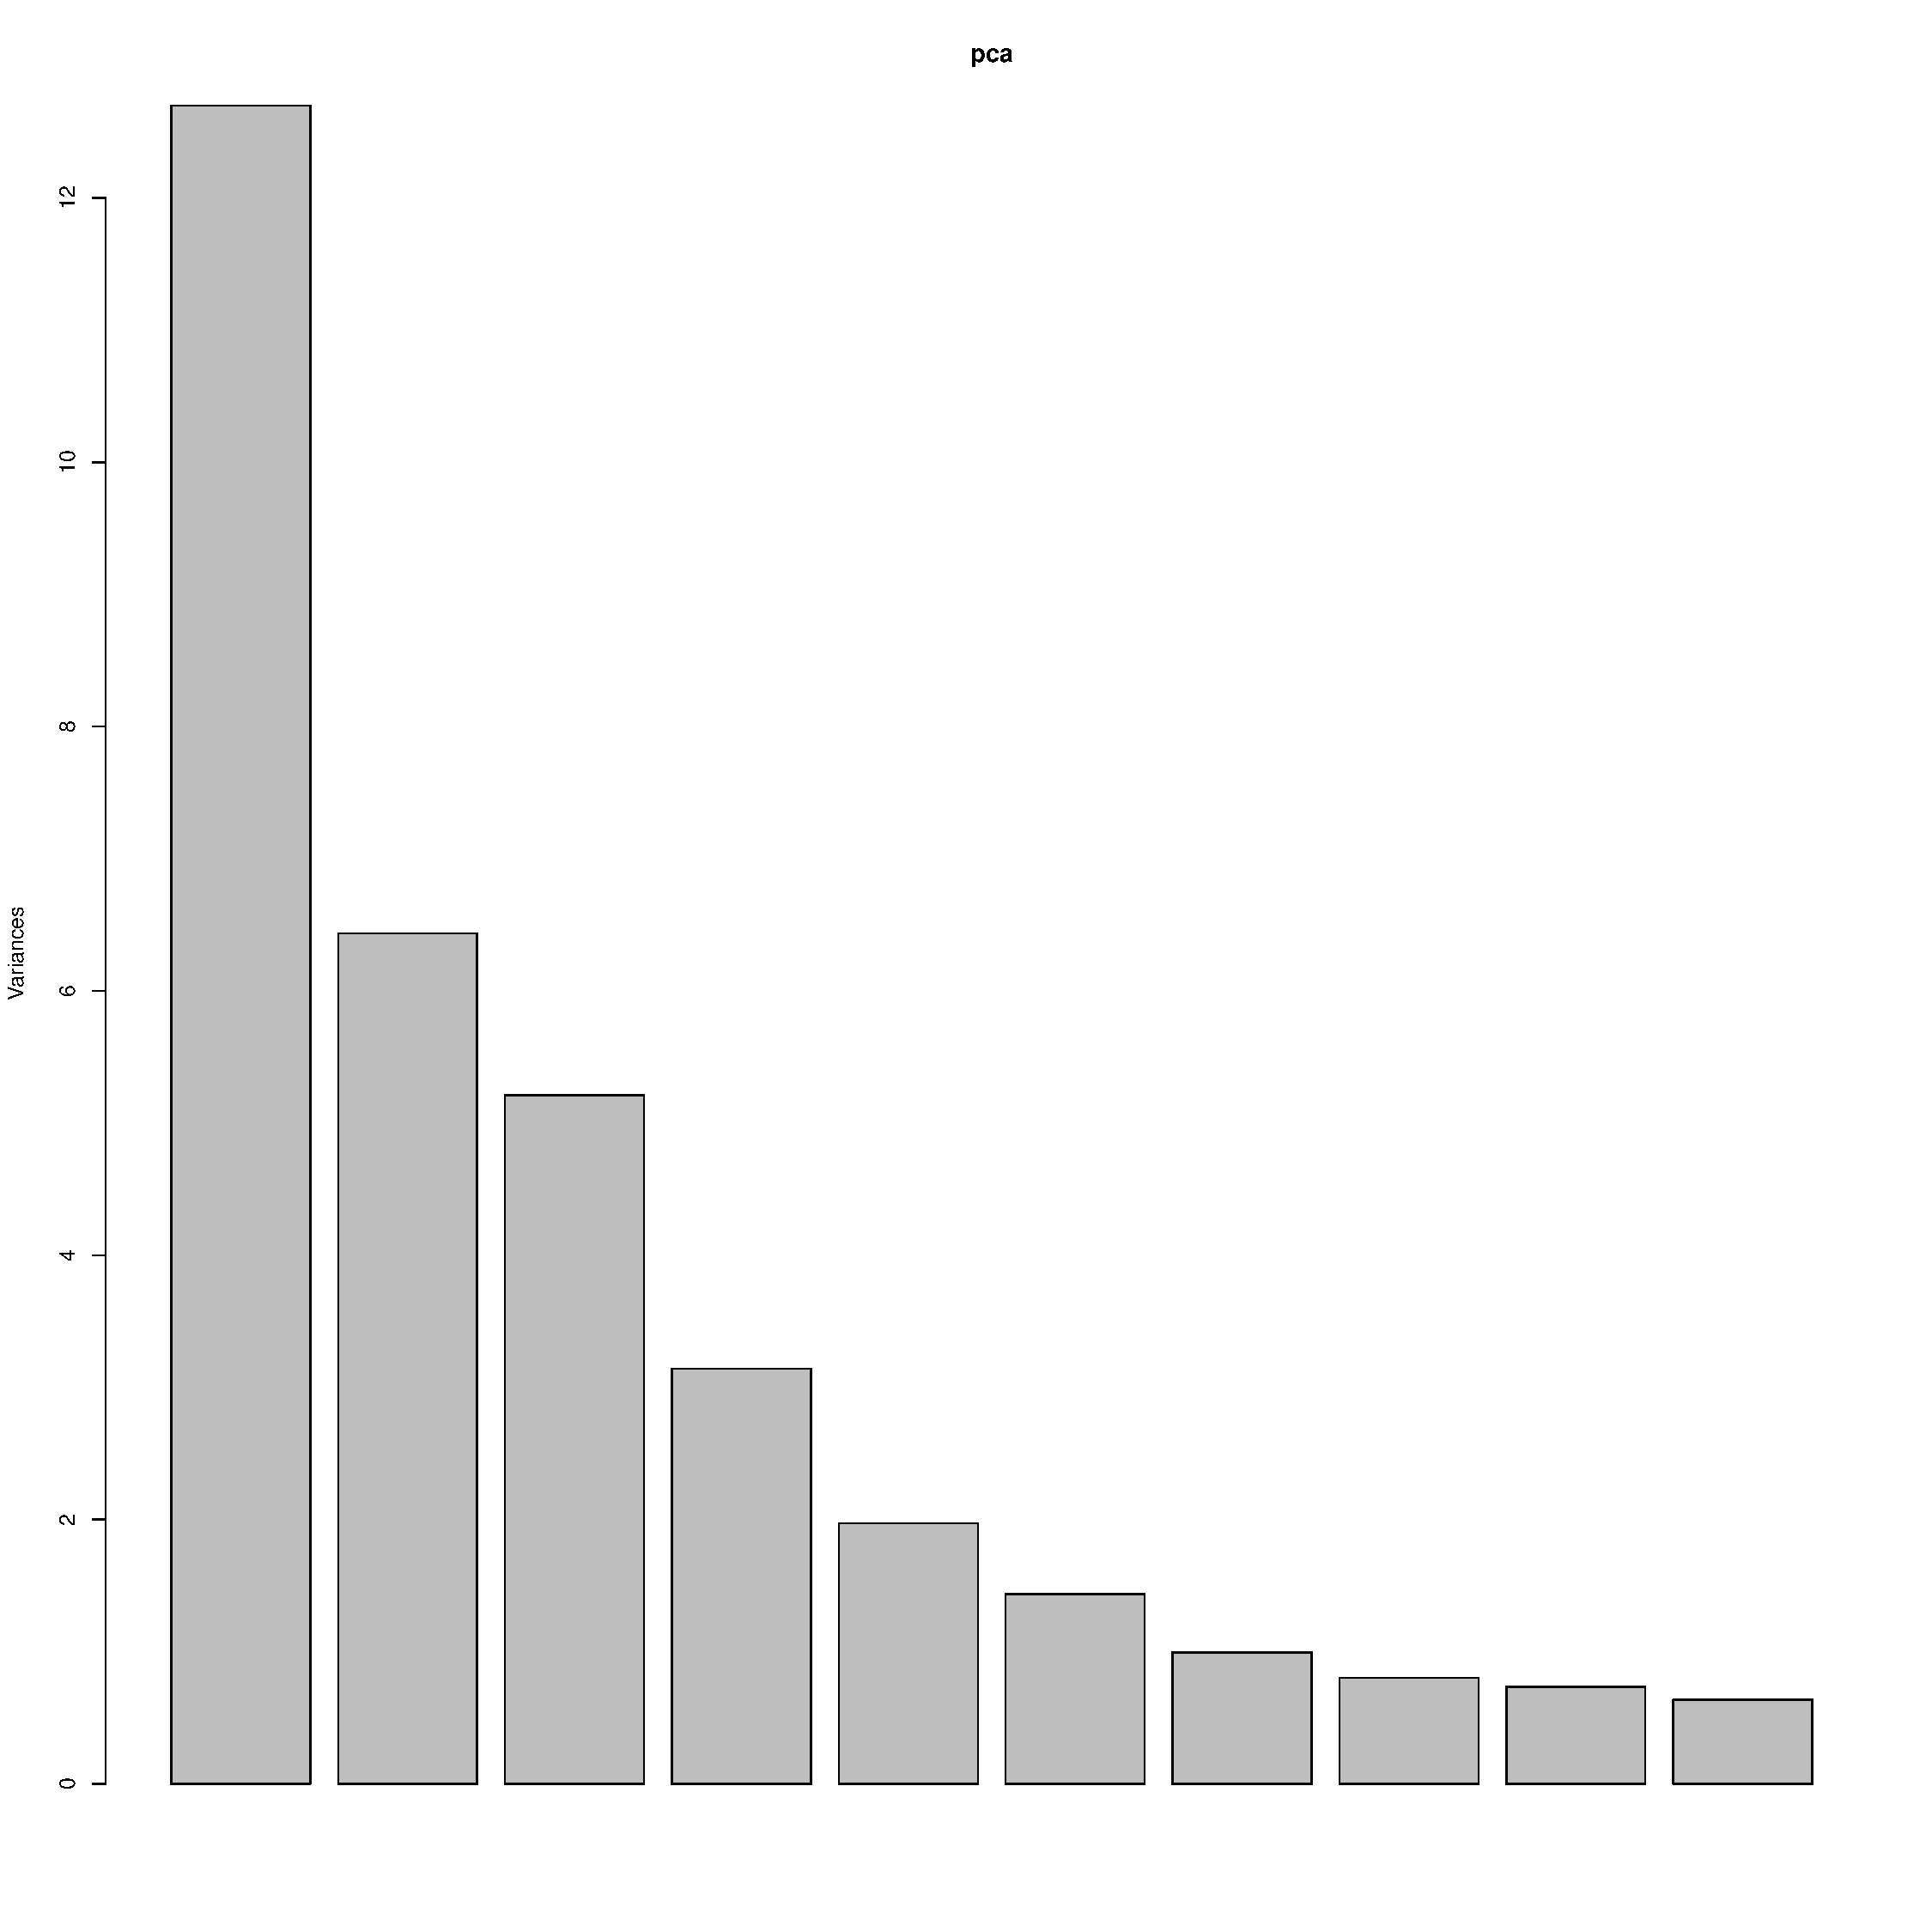
\includegraphics[width = 0.44 \textwidth , page=1]{./Results/pca_scaled.pdf}
	\caption{نمودار ستونی میزان تغییرات بیان شده توسط هر یک از مولفه‌های \lr{PCA} پس از \lr{Scale} شدن}
	\label{fig:pcahist2}
\end{figure}

\begin{figure}[h!]
	\centering	
	\includegraphics[width = 0.44\textwidth , page =2]{./Results/pca_scaled.pdf}
	\caption{نمودار نقطه‌ای (\lr{scatterplot}) داده‌ها براساس دو مولفه با بیش‌ترین اهمیت پس از \lr{Scale} شدن}
	\label{fig:pcadot2}
\end{figure}
\newpage

حال با کمک مولفه \lr{rotation} در \lr{PCA}، نمودار مربوط به نمونه‌های مختلف را با رنگ‌های مختلف رسم می‌کنیم.

\begin{latin}
	\begin{lstlisting}[language=R]
		pcar <- data.frame(pca$rotation[,1:3] , group = gr)
		ggplot(pcar , aes(PC1 , PC2 , color = group , size = 4)) + geom_point()+ theme_bw()
	\end{lstlisting}
\end{latin} 

شکل نمودار در زیر آورده شده است:

\begin{figure}[h!]
	\centering	
	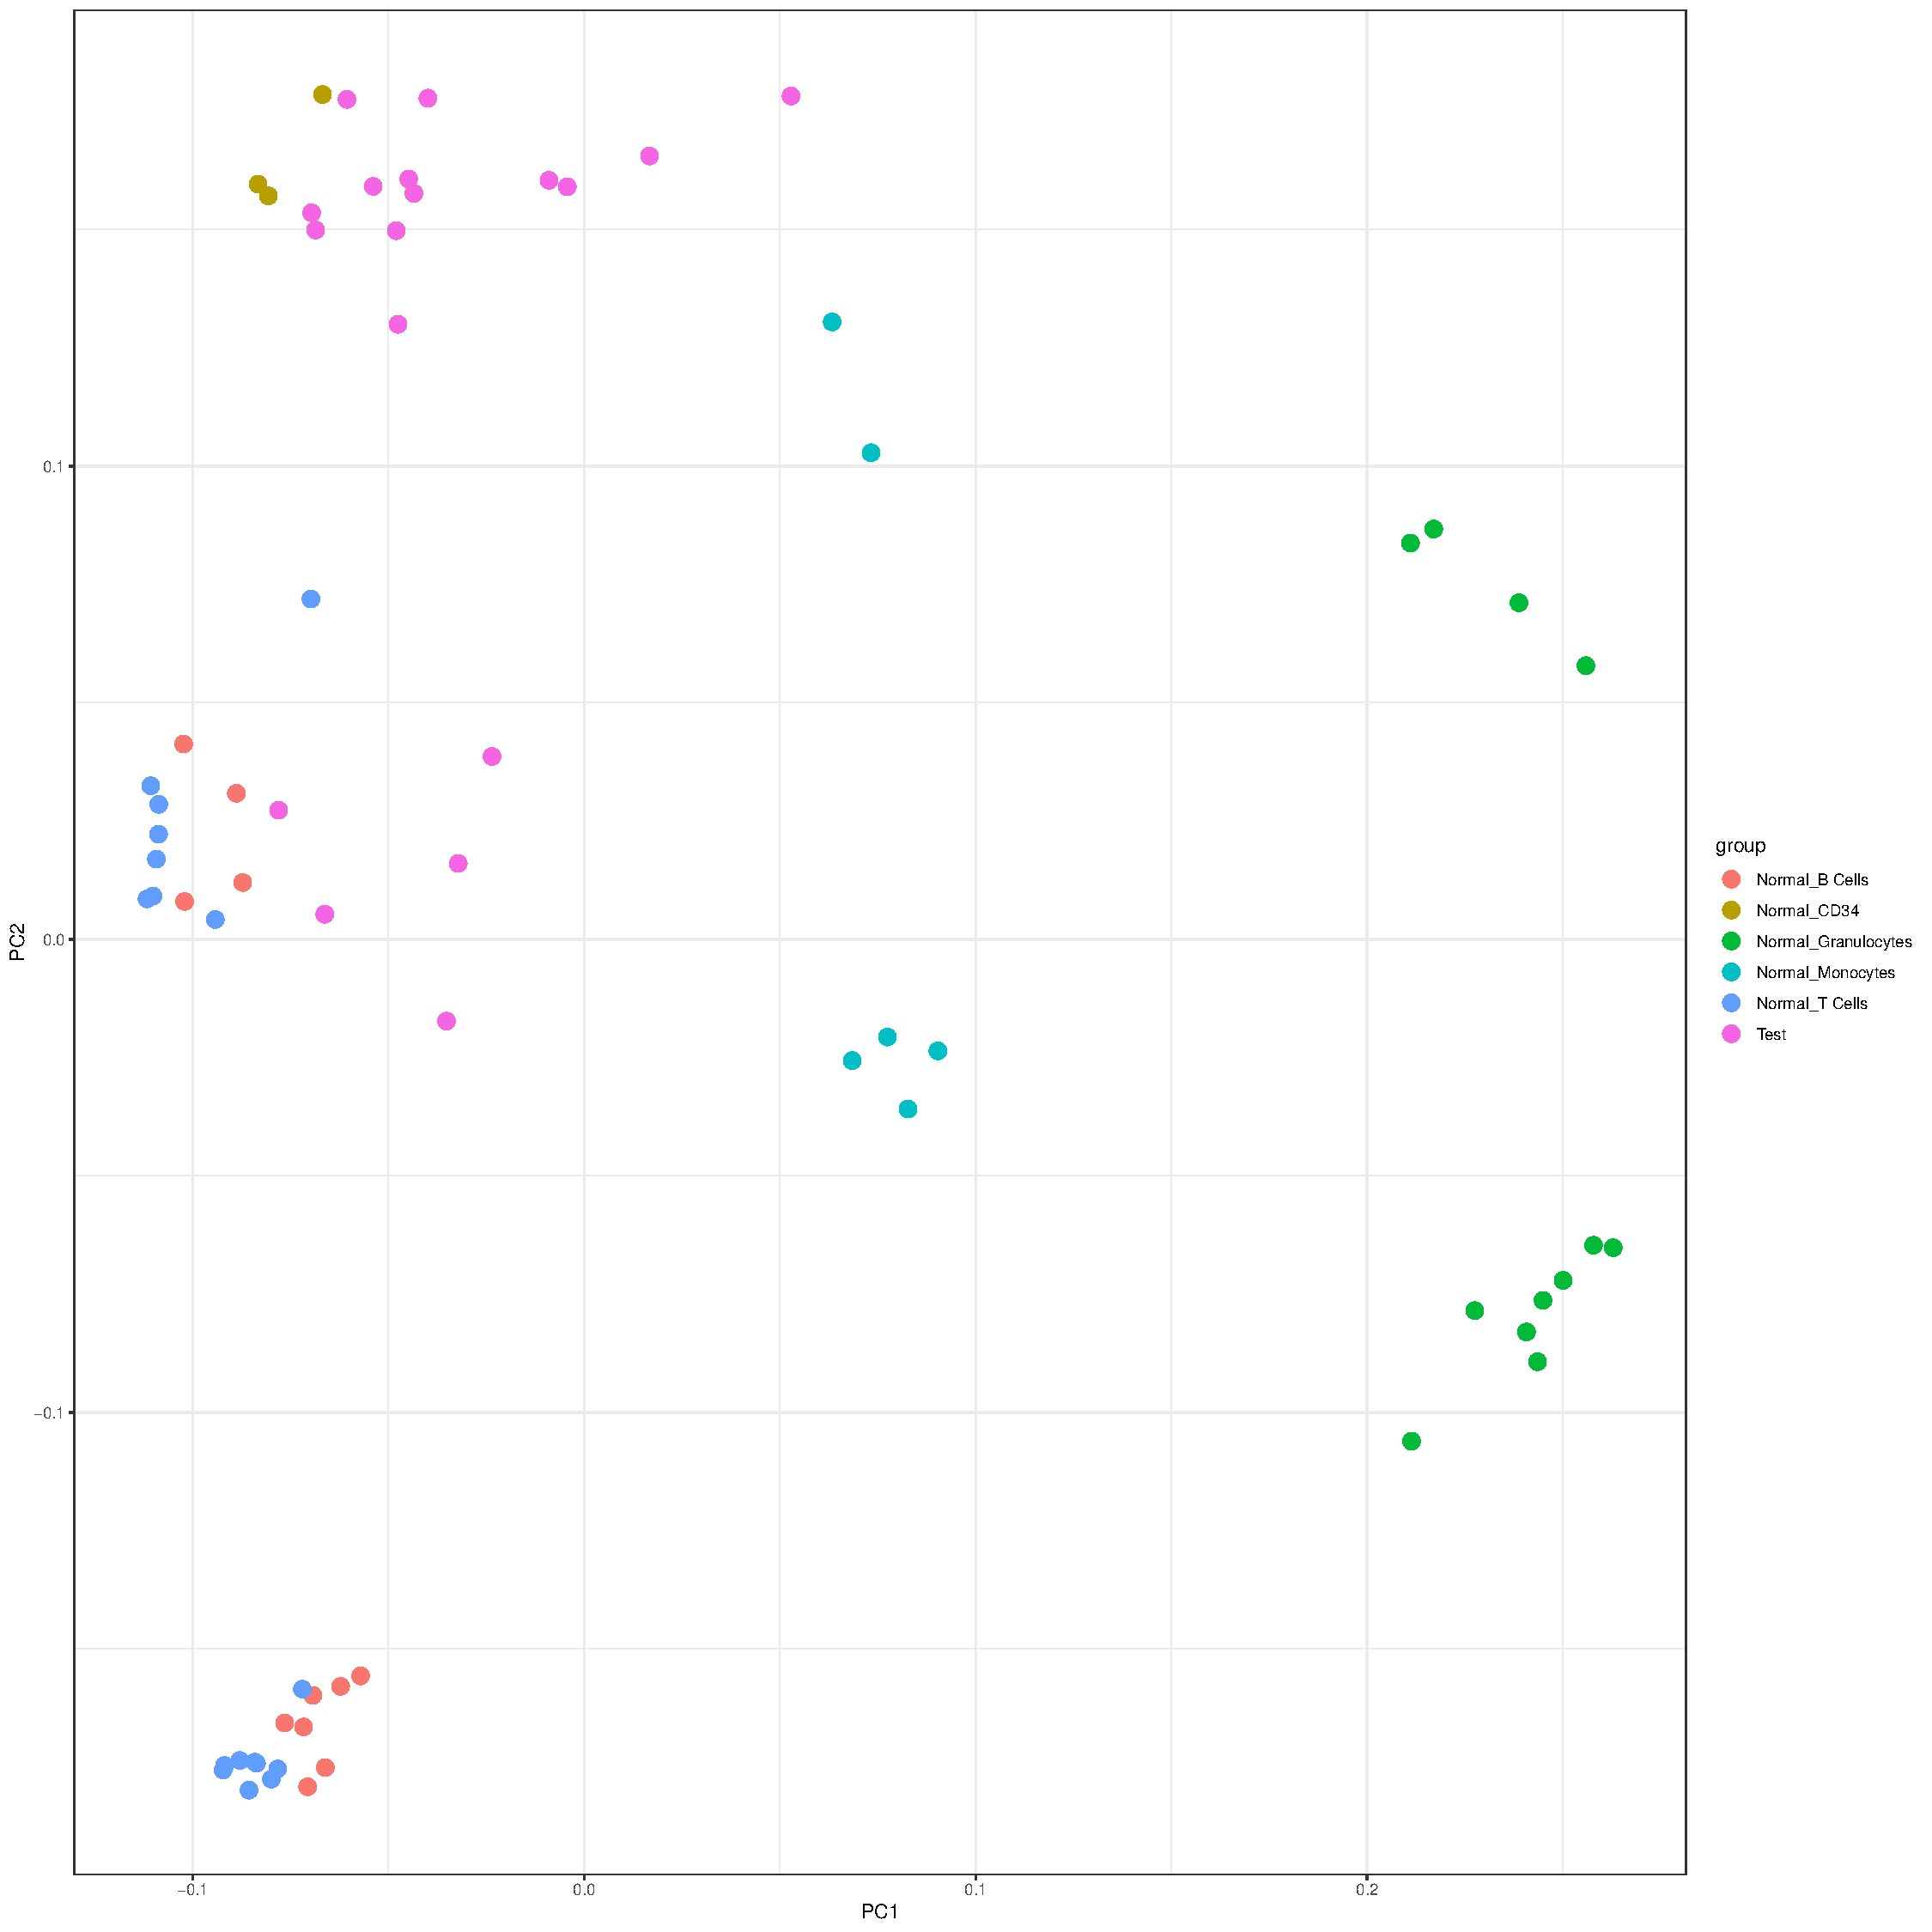
\includegraphics[width = 0.75 \textwidth ]{./Results/PCA_Samples.pdf}
	\caption{نمودار \lr{Scatterplot} نمونه‌ها براساس دو مولفه اصلی در \lr{PCA} و رنگ شده براساس نوع مولفه}
	\label{fig:pcasamples}
\end{figure}





\subsection{نمودار همبستگی \lr{Heatmap}}

برای رسم نمودار همبستگی و Heatmap از کد زیر استفاده می‌کنیم:

\begin{latin}
	\begin{lstlisting}[language=R]
		pheatmap(cor(expr), labels_row = gr, labels_col = gr, color = bluered(256), border_color = NA)
	\end{lstlisting}
\end{latin}
نتیجه بدین صورت خواهد بود:






\begin{figure}[h!]
	\centering	
	
\includegraphics[width = 1.1 \textwidth ]{./Results/CorHeatmap.pdf}
	\caption{نمودار \lr{Heatmap} همبستگی بین نمونه‌های مختلف}
	\label{fig:heat}
\end{figure}


\newpage

\subsection{پیدا کردن تفاوت‌های بیان ژن در سلول بیماران و سلول‌های سالم}

با توجه به شکل‌های \ref{fig:pcasamples} و \ref{fig:heat} می‌بینیم که سلول‌های تست به سلول‌های \lr{CD34} نزدیک‌‌تر هستند. برای همین ابتدا آن دسته از سلول‌های تست که به \lr{CD34} نزدیک‌تر هستند را با نماد دیگری در گروه‌ها مشخص می‌کنیم. با توجه به شکل \ref{fig:pcasamples} می‌بینیم که برای این دسته مولفه \lr{PC2} بیش از $0.11$ و \lr{PC1} آن‌ها کمتر از $-0.025$ است. آن‌ها را با نماد
\lr{"AML\_Near\_CD34"}
مشخص می‌کنیم. کد این کار در زیر آورده شده است:

\begin{latin}
\begin{lstlisting}[language=R]
gr2 <- gr
gr2[which(pcar$PC2 > 0.11 & pcar$group == "Test")] <-
"AML_Near_CD34"
gr2 <- factor(gr2)
gset$description <- gr2
\end{lstlisting}
\end{latin}

دلیل استفاده از تابع \lr{factor} این است که عبارات درون \lr{gr2} صرفا به عنوان یکسری رشته معمولی نباشند و به عنوان سطوح مختلف از یک متغیر مشخص در نظر گرفته شوند.

پس از آن باید یک ماتریس بسازیم که برای هر نمونه، مشخص کند که در کدام دسته قرار دارد. این ماتریس را برای این که بتوانیم پس از آن از قابلیت \lr{linear model fit} کتابخانه \lr{Limma} استفاده کنیم، باید به صورت
 \lr{One-Hot}
  بسازیم(این اسم از درس مدار منطقی گرفته شده است). یعنی برای هر نمونه، ستون تمامی دسته‌ها وجود داشته باشد و دسته مربوط مقدار $1$ و مابقی مقدار $0$ داشته باشند. ضمنا در نام یکسری از دسته‌ها اسپیس وجود دارد که برای این که در پکیج‌های بعدی به مشکل نخوریم، این اسپیس با \_ جایگزین شده است. در کد پایین توجه کنید که تابع \lr{str\_replace} مربوط به کتابخانه \lr{stringr} است.



\begin{latin}
	\begin{lstlisting}[language=R]
	onehot <- model.matrix(~ description + 0, gset)
	colnames(onehot) <- levels(gr2)
	
	colnames(onehot) <-
	c(sapply(colnames(onehot) , function(x)
	str_replace(x, " ", "_")))
	\end{lstlisting}
\end{latin}



بعد از این ابتدا یک مدل خطی
\LTRfootnote{Linear Model}
روی داده ها \lr{Fit}
 می‌کنیم. سپس تفاوت بین بیان‌ژن‌های دسته سلول‌های بیمار و دسته سلول‌های \lr{CD34} را بدست می‌آوریم. پس از آن از طریق یک مدل بیزین، مدل جدیدی را Fit می‌کنیم. در این مدل بیزین، دانش پیشین ما بر این فرض است که حدود $1$ درصد ژن‌ها باید تفاوت بیان نشان بدهند. این مدل براساس این دانش \lr{Posterior}، توزیع نهایی را بدست آورده و در نهایت جدول نهایی که شامل مواردی نظیر  \lr{Adjusted P Value} و همچنین \lr{log Fold Change} برای ژن‌های مختلف است را بدست می‌آورد. در این جدول اطلاعات دیگری هم موجود است ولی ما تنها نام و نشانه ژن‌ها و همچنین \lr{adj.P.Val} و \lr{logFC} را برای مرحله بعد نیاز داریم.(در ویدیو دکتر شریفی زارچی هم همین داده ها نگه داشته شدند)



 
 \begin{latin}
 	\begin{lstlisting}[language=R]
 		fit <- lmFit(gset , onehot)
 		
 		contrast <-
 		makeContrasts(AML_Near_CD34 - Normal_CD34 , levels = onehot)
 		
 		fit2 <- contrasts.fit(fit , contrast)
 		fit2 <- eBayes(fit2 , 0.01)
 		tT <- topTable(fit2,
 		adjust = "fdr",
 		sort.by = "B" , number = Inf)
 		tT2 <- subset(tT , select = c("Gene.symbol" , "Gene.id", "Gene.title", "adj.P.Val"  , "logFC"))
 			\end{lstlisting}
 \end{latin}



با توجه به این که \lr{logFC} بزرگتر از $1$ نشان دهنده تفاوت بیش از دوبرابری در بیان بیش‌تر یک ژن و کمتر از $-1$ نشان دهنده تفاوت بیش از دو برابری در بیان کمتر یک ژن است، از این طریق و با توجه به \lr{adj.P.Val} کمتر از $0.05$ ژن‌هایی که تفاوت بیان معنی دار داشتند را بدست می‌‌‌آوریم. از آن‌جایی که بعضی از ژن‌ها چند نماد دارند که با "///`` جدا شده‌اند،‌ از همه این نماد‌ها در جواب استفاده می‌کنیم. همه این ژن‌ها در دو فایل مربوطه در پوشه \lr{Results} ذخیره شده‌اند.




 \begin{latin}
	\begin{lstlisting}[language=R]
aml.up <- subset(tT2, logFC > 1 & adj.P.Val < 0.05)
aml.up.genes <-unique( as.character(
strsplit2( (aml.up$Gene.symbol),"///")))
aml.down <- subset(tT2, logFC < -1& adj.P.Val < 0.05)
aml.down.genes <- unique(as.character(
strsplit2( (aml.down$Gene.symbol),"///")))
	\end{lstlisting}
\end{latin}



\section{تحلیل \lr{Gene Ontology} و \lr{Pathways} به کمک \lr{Enrichr}}

\subsection{تحلیل ژن‌ها با بیان بالاتر در سلول‌های بیمار}
\subsubsection{تحلیل \lr{Pathway}}
برای تحلیل از \lr{Enrichr} استفاده می‌کنیم \cite{enrichr,enrichr2}. با تحلیل ژن‌هایی که در بیماران بیان بالاتری داشته اند، در میان Pathway ها براساس مجموعه \lr{WikiPathways 2021 Human} موارد زیر قابل توجه بودند:
\begin{latin}
\begin{itemize}
	\item  {TYROBP Causal Network} : $APV = 2.264 \times 10^{-8}$
	
	\item  {Microglia Pathogen Phagocytosis Pathway}: $APV = 1.143 \times 10^{-9}$ 
	
	\item {Platelet-mediated interactions with vascular and circulating cells}  : $APV = 0.0002054$ 
\end{itemize}
\end{latin}
البته موارد دیگری هم هستند ولی این موارد، از نظر موضوعی هم در مقالات مرتبط با \lr{AML} به خوبی بررسی شده اند. (جدول کامل در کنار این فایل قرار دارد)

همانطور که مشاهده میشود، اغلب ژن هایی که. در این مسیر های زیستی قرار دارند مربوط به مکانیسم های ایمنی بدن هستند، برای مثال ژن \lr{CD84} که در مسیر زیستی سوم بالا قرار دارد و این ژن یک گلیکوپروتئین غشایی را کد می کند که عضوی از خانواده مولکول فعال کننده لنفوسیت سیگنال
\lr{(SLAM)}
 است. این خانواده زیرمجموعه ای از ابرخانواده گیرنده سطح سلولی
\lr{CD2}
  بزرگتر 
 \lr{Ig}
   را تشکیل می دهد. پروتئین کدگذاری شده یک مولکول چسبندگی هموفیل است که در انواع سلول های ایمنی متعدد بیان می شود و در تنظیم سیگنال دهی با واسطه گیرنده در آن سلول ها نقش دارد. پیوند متناوب منجر به انواع رونوشت های متعدد می شود.
 \cite{ch1, ch2}
 
 همچنین برای مسیر زیستی دوم، برای ژن 
 \lr{C3}
 میبینیم که این ژن هم در مکانیسم های ایمنی بدن نقش داشته است، این ژن دستورالعمل هایی را برای ساخت پروتئینی به نام جزء مکمل 
\lr{3}
  (یا 
 \lr{C3}
  ) ارائه می دهد. این پروتئین نقش کلیدی در بخشی از پاسخ ایمنی بدن به نام سیستم مکمل دارد. سیستم کمپلمان گروهی از پروتئین‌ها است که با هم کار می‌کنند تا مهاجمان خارجی (مانند باکتری‌ها و ویروس‌ها) را از بین ببرند، التهاب را تحریک کنند و بقایای سلول‌ها و بافت‌ها را حذف کنند.
\cite{ch3}

در مسیر زیستی سوم نیز ژن 
\lr{NCF4}
 قرار دارد که دستورالعمل هایی را برای ساخت پروتئینی به نام فاکتور سیتوزولی نوتروفیل 
\lr{4}
  (همچنین به نام 
 \lr{p40-phox}
  ) ارائه می دهد. این پروتئین یک بخش (زیر واحد) از گروهی از پروتئین ها است که یک کمپلکس آنزیمی به نام 
\lr{NADPH}
   اکسیداز را تشکیل می دهد که نقش اساسی در سیستم ایمنی دارد. به طور خاص، 
\lr{NADPH}
    اکسیداز در درجه اول در سلول های سیستم ایمنی به نام فاگوسیت ها فعال است. این سلول ها مهاجمان خارجی مانند باکتری ها و قارچ ها را می گیرند و از بین می برند. همچنین تصور می شود 
\lr{NADPH}
     اکسیداز فعالیت سلول های ایمنی به نام نوتروفیل ها را تنظیم می کند. این سلول ها در تنظیم پاسخ التهابی برای بهبود بهینه و کاهش آسیب به بدن نقش دارند.
\cite{ch4}

همچنین تحلیل ژن‌هایی که در بیماران بیان پایین‌تری داشته اند، در میان Pathway ها براساس مجموعه \lr{WikiPathways 2021 Human} موارد زیر قابل توجه بودند:
\begin{latin}
\begin{itemize}
	\item  {Cholesterol metabolism (includes both Bloch and Kandutsch-Russell pathways) WP4718} : $APV = 0.001796$
\end{itemize}
\end{latin}
موارد دیگر \lr{APV} بیشتری از 
\lr{0.05}
 داشتند و معنادار محسوب نمیشدند، مجددا جدول کامل فرستاده شده است.
در ادامه تصاویر این Pathway ها قرار گرفته است. همانطور که مشاهده میشود، تقریبا در همه این مسیر های زیستی، مکانیسم های ایمنی بدن قرار دارند که تاثیر پذیرفته اند. مخصوصا درمورد مسیر های زیستی‌ای که به افزایش بیان یک ژن مربوط بوده‌اند.
\newpage
\begin{figure}[h!]
	\centering	
	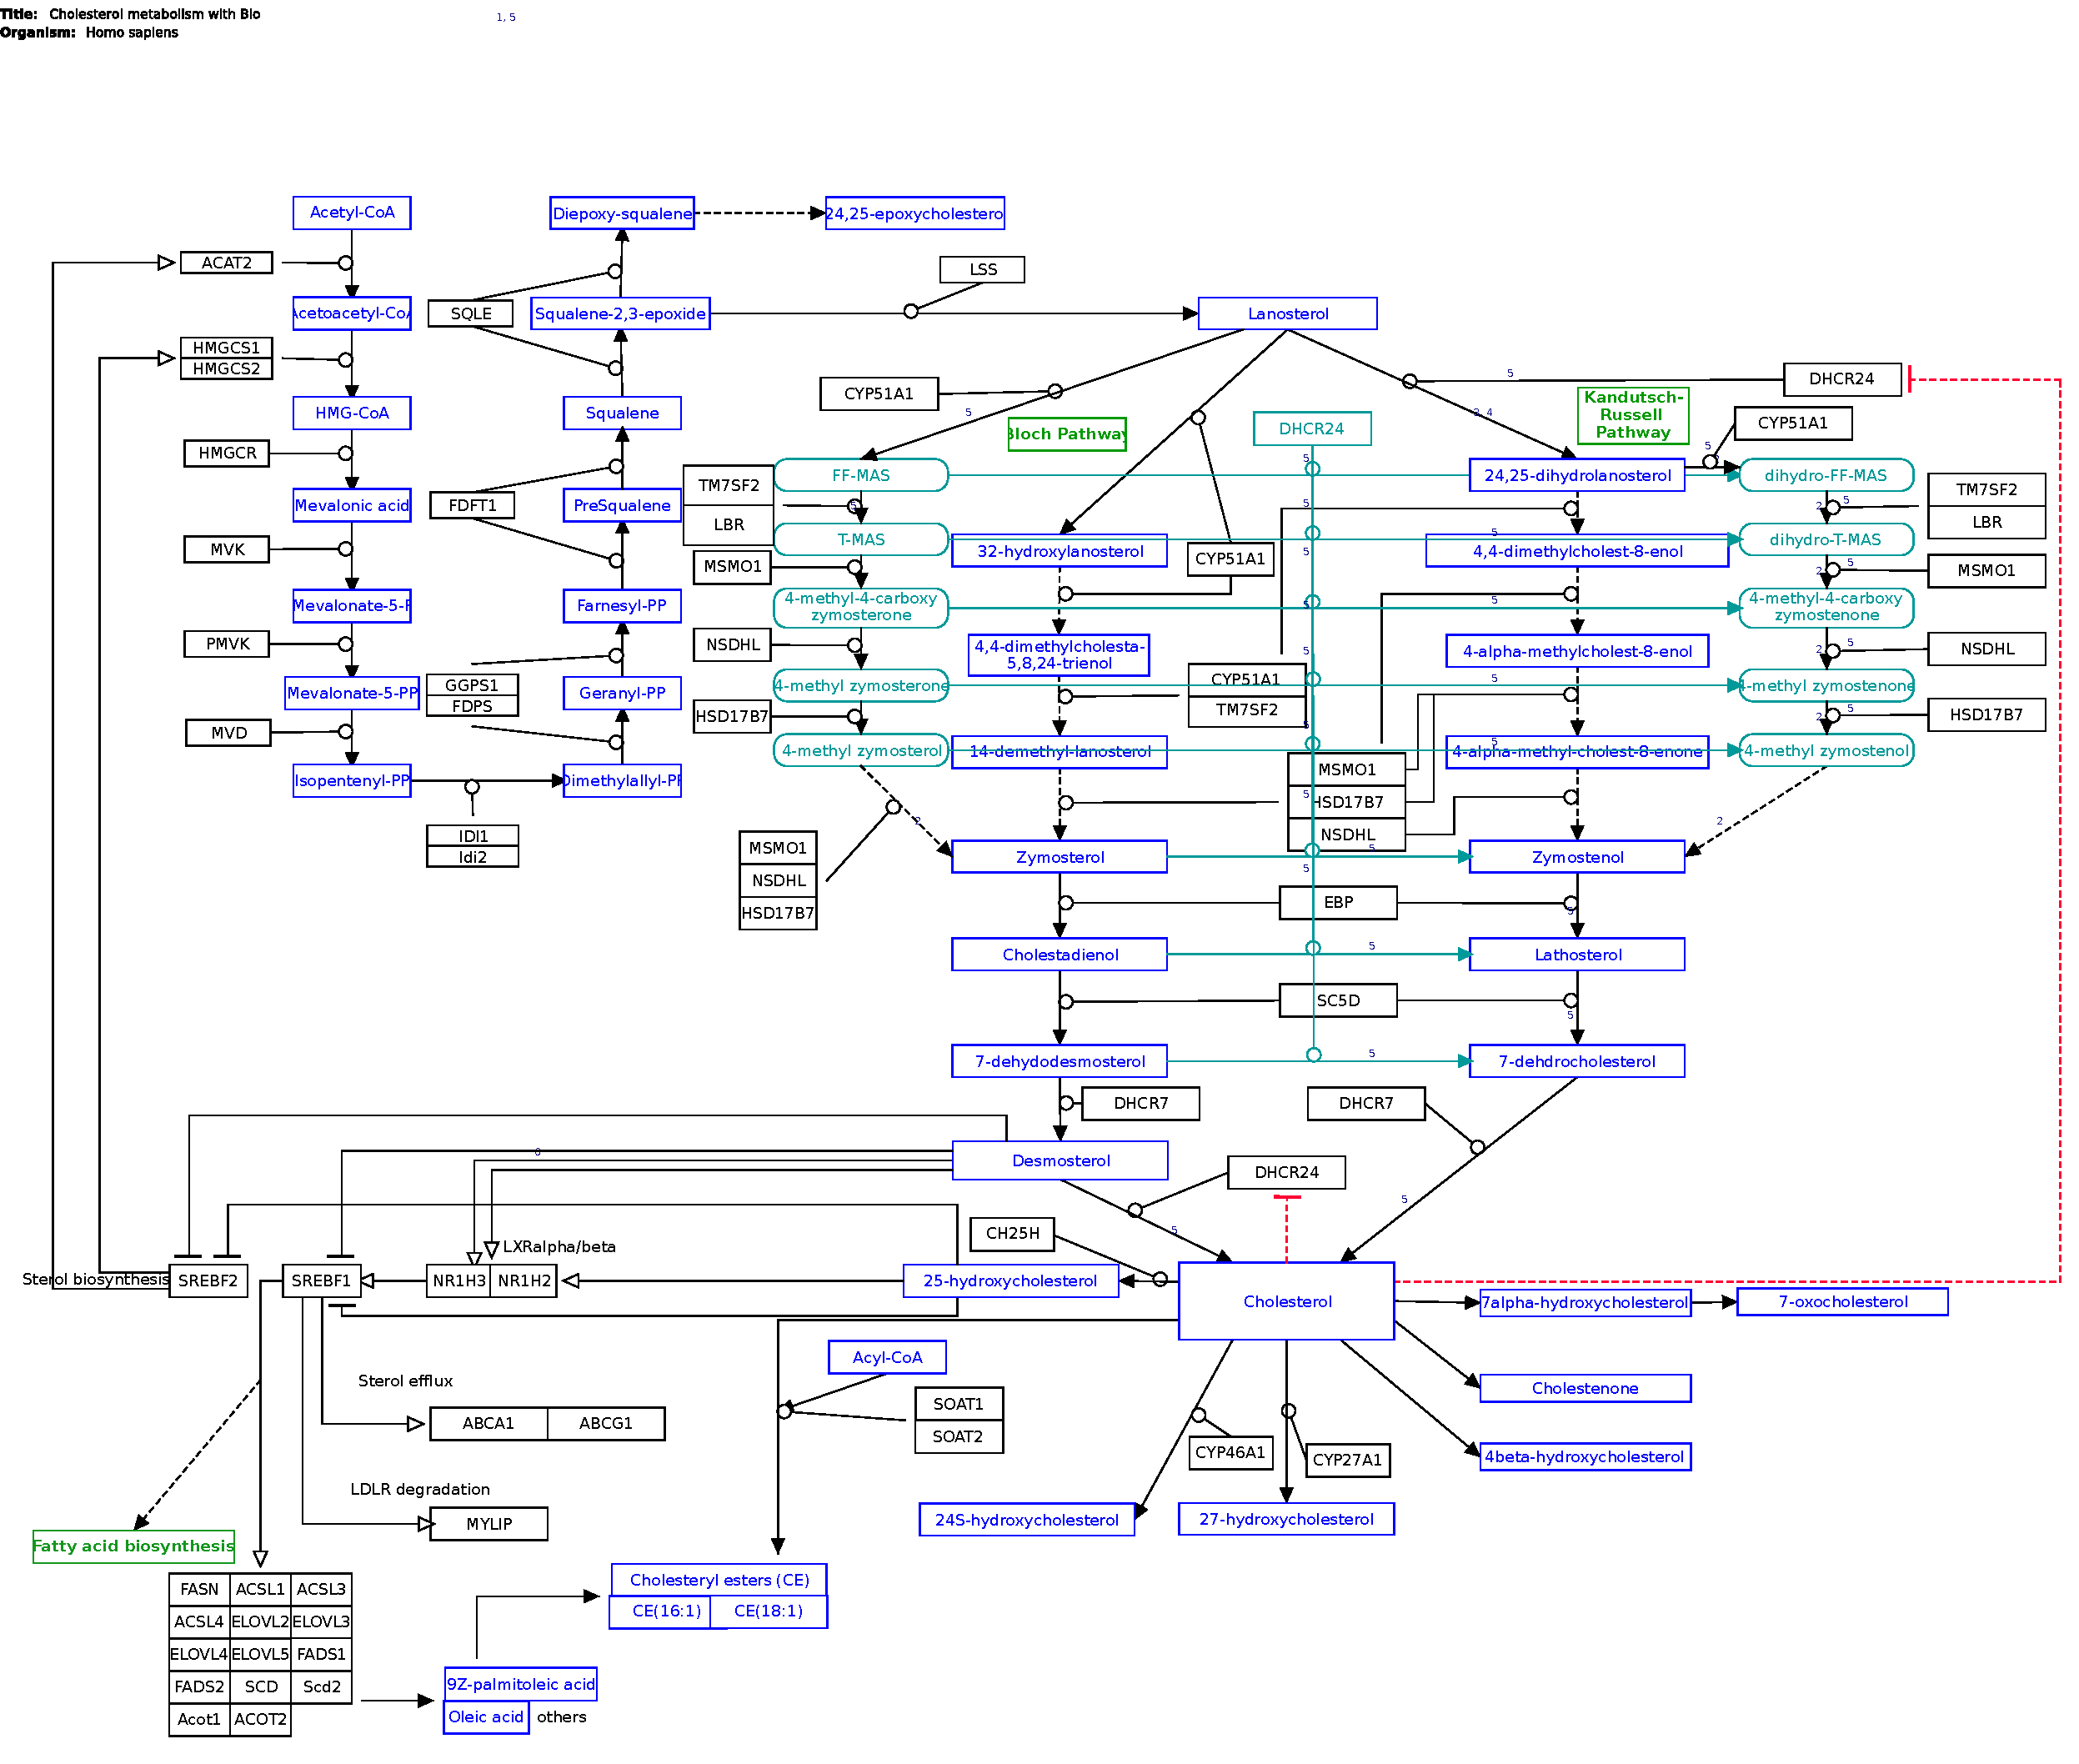
\includegraphics[width = 1.1 \textwidth ]{./Results/path5.pdf}
	\caption{
	\lr{pathway}
مربوط به 
\lr{Cholesterol metabolism}
}
	\label{fig:path_down}
\end{figure}

\begin{figure*}[h!]
\begin{minipage}{.5\linewidth}
	\centering
	\subfloat[]{\label{path_up:a}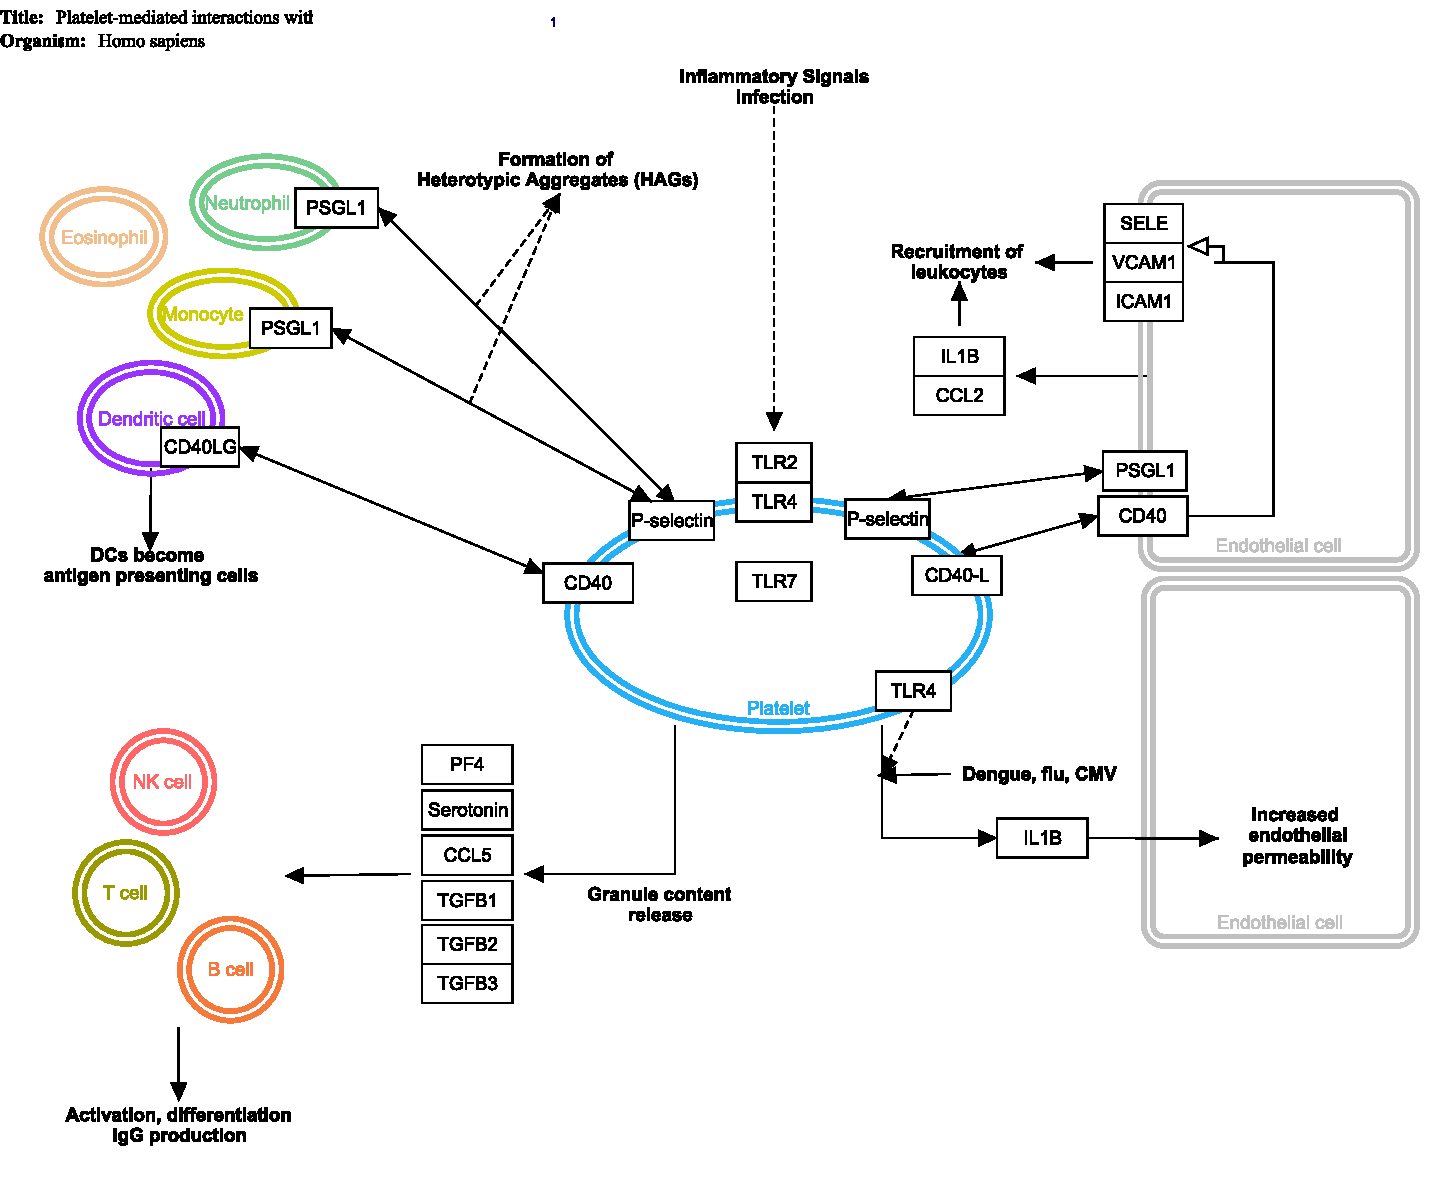
\includegraphics[width=1.0 \textwidth]{./Results/path.pdf}}
\end{minipage}%
\begin{minipage}{.5\linewidth}
	\centering
	\subfloat[]{\label{path_up:b}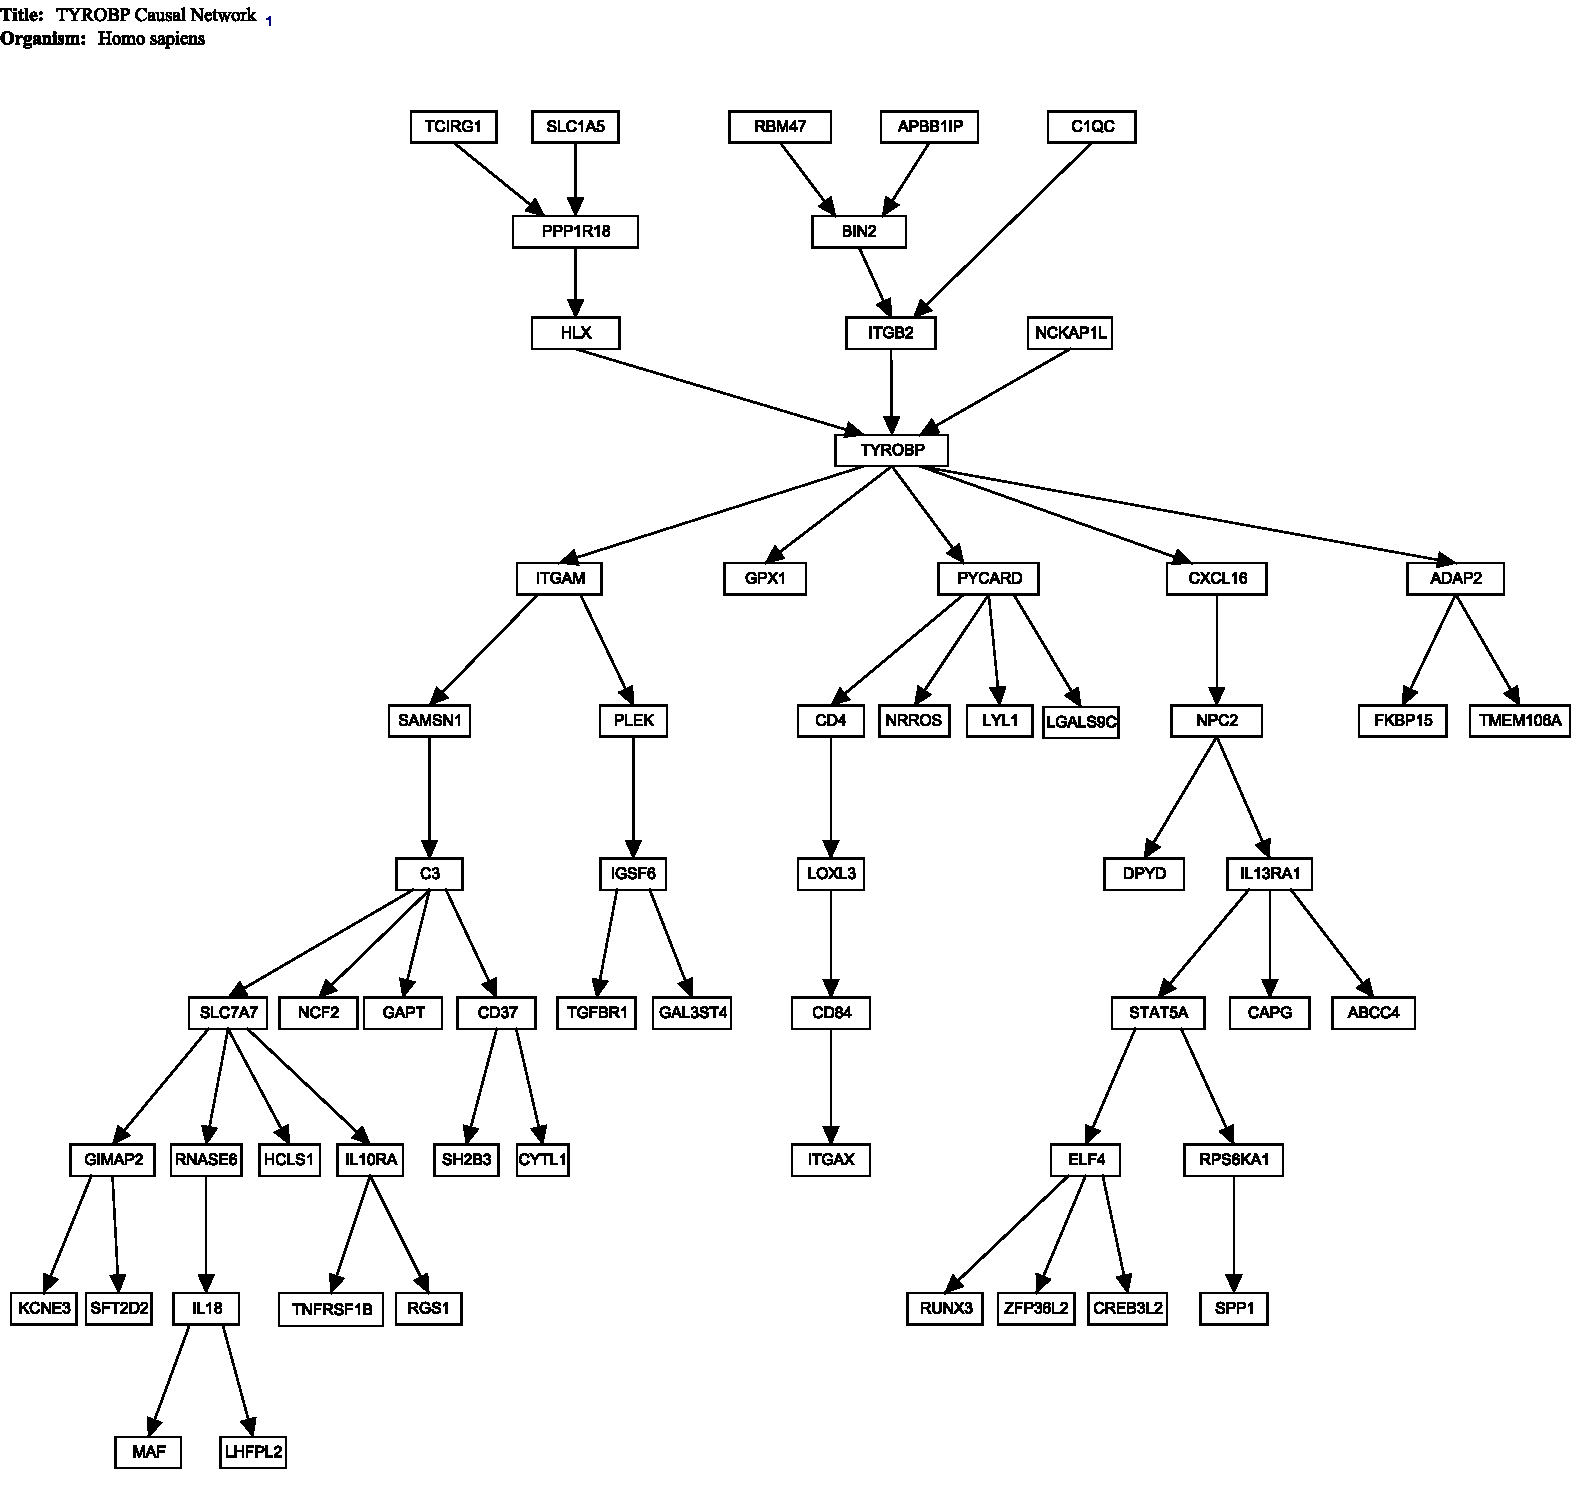
\includegraphics[width=1.0 \textwidth]{./Results/path3.pdf}}
\end{minipage}\par\medskip
\centering
\subfloat[]{\label{path_up:c}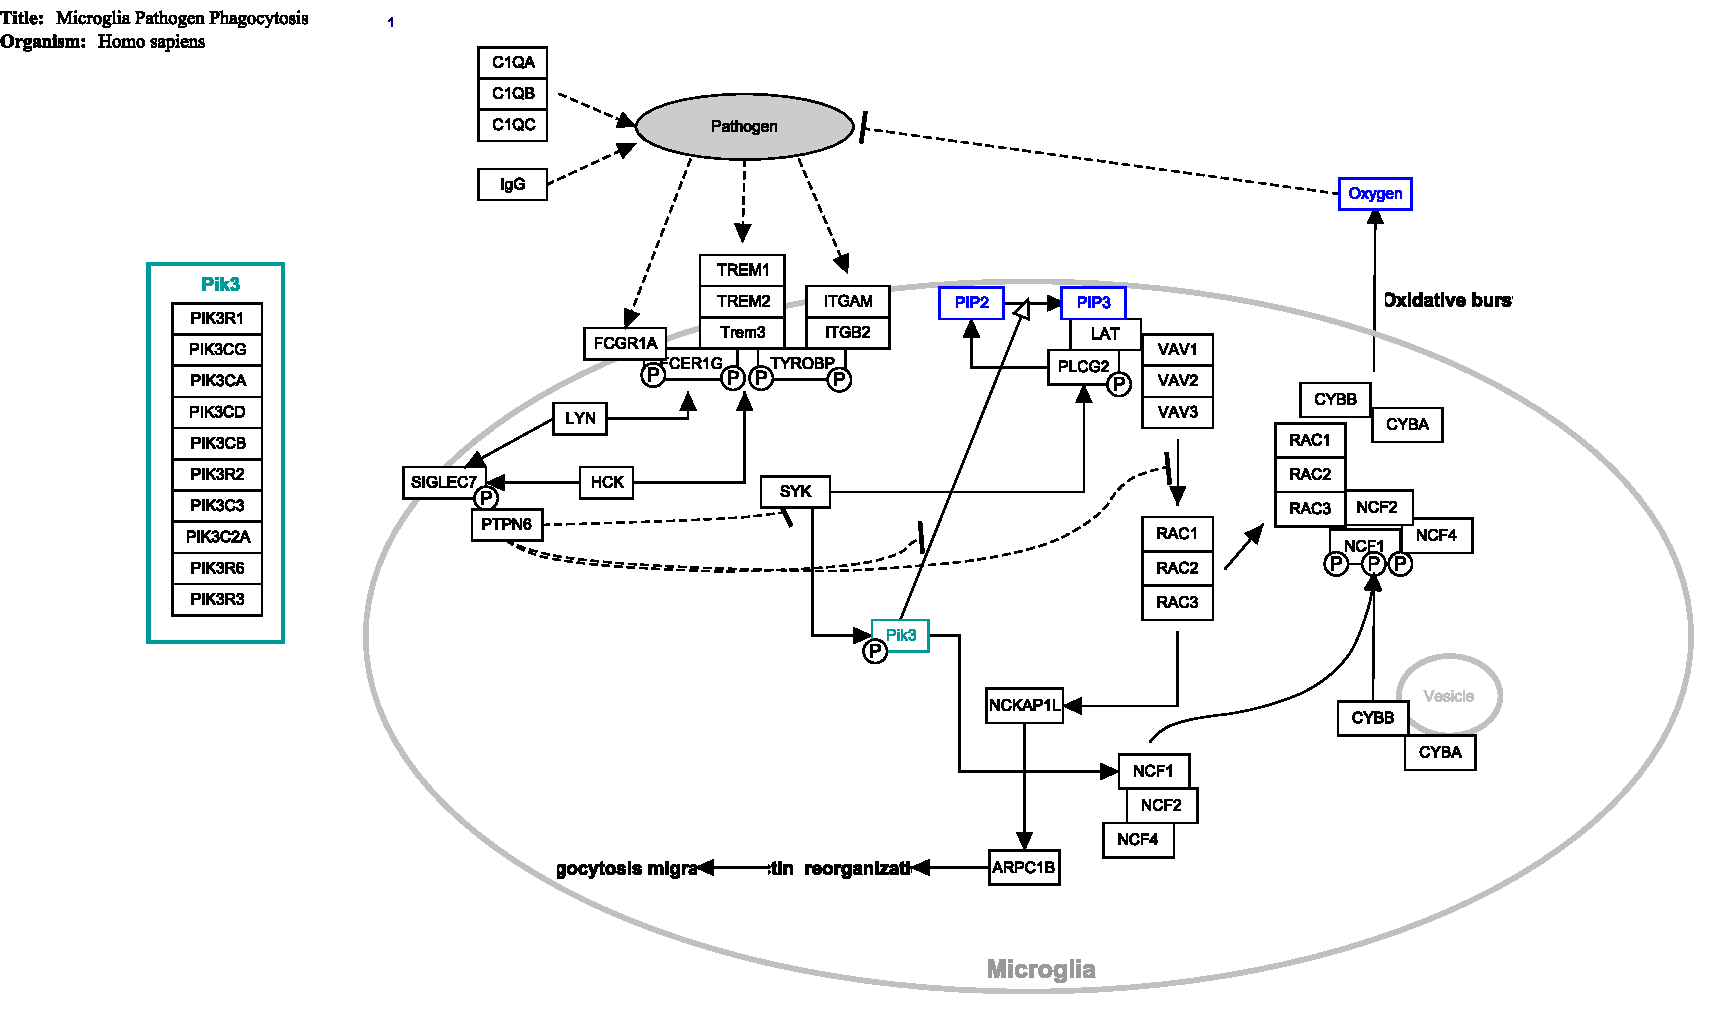
\includegraphics[width=1.0 \textwidth]{./Results/path2.pdf}}
\label{fig:path_up}
\caption{
قسمت (آ) مربوط به \lr{{Platelet-mediated interactions with vascular and circulating cells}} قسمت (ب) مربوط به \lr{ {TYROBP Causal Network}} و قسمت (ج) مربوط به \lr{{Microglia Pathogen Phagocytosis Pathway}} است.
}
\end{figure*}



\newpage

\subsubsection{تحلیل\lr{ Gene Ontology}}


در زمینه \lr{Molecular Function}، موارد زیر قابل توجه هستند:

\begin{latin}
	\begin{itemize}
		\item  {Toll-like receptor binding (GO:0035325)} : $APV =0.003139$
		
		\item  {kinase binding  (GO:0019900)}: $APV = 1.846 \times 10^{-7}	$ 
		
		\item {aryl sulfotransferase activity (GO:0004062)}  : $APV = 0.005231$ 
	\end{itemize}
\end{latin}

یرنده های شبه تلفن (
\lr{TLRs}
) دسته ای از گیرنده های تشخیص الگو (
\lr{PRRs}
) هستند که پاسخ ایمنی ذاتی را با سنجش الگوهای مولکولی حفظ شده برای شناسایی اولیه یک پاتوژن از طریق ایمنی آغاز می کنند.

برای دو مورد دیگر هم قالات زیادی نوشته شده‌اند که آنهارا به سیستم ایمنی پیوند میزنند. در واقع هر سه اینها با سیستم ایمنی ارتباط دارند.



در زمینه ‌\lr{Biological Process} موارد زیر قابل توجه هستند:
\begin{latin}
	\begin{itemize}
		\item  {neutrophil activation involved in immune response (GO:0002283)} : $APV =4.830 \times 10^{-37}$
		
		\item  {neutrophil degranulation (GO:0043312)}: $APV =6.631 \times 10^{-37}	$ 
		
		\item {neutrophil mediated immunity (GO:0002446)}  : $APV = 2.158 \times 10^{-37}$ 
	\end{itemize}
\end{latin}

این بار هرسه عبارات شامل نوتروفیل هستند پس این سه هم واضحا به سیستم ایمنی اشاره دارند و نتیجه مجددا مشابه قسمت های قبلی است.


در زمینه \lr{Cellular Component} موارد زیر قابل توجه هستند:
\begin{latin}
	\begin{itemize}
		\item  {specific granule membrane (GO:0035579)} : $APV =7.816 \times 10^{-14}$
		
		\item  {specific granule (GO:0042581)}: $APV =2.843 \times 10^{-14}	$ 
		
		\item {tertiary granule (GO:0070820)}  : $APV = 3.434 \times 10^{-14}$ 
	\end{itemize}
\end{latin}

گرانول‌ها مخلوطی از مولکول‌های سیتوتوکسیک، از جمله بسیاری از آنزیم‌ها و پپتیدهای ضد میکروبی را ذخیره می‌کنند که توسط فرآیندی به نام 
\lr{degranulation}
 به دنبال فعال شدن گرانولوسیت توسط یک محرک ایمنی آزاد می‌شوند. ... گرانول های اختصاصی به «گرانول های ثانویه» نیز معروف هستند. همانطور که مشاهده میشود هرسه اینها هم به سیستم ایمنی اشاره میکنند و با آن ارتباط دارند.
 
 بنابراین با نتایج بدست آمده میتوان گفت تحلیل های ما خوب و درست بوده اند چراکه بسیار منطقی است که سرطان موجب اختلال در سیستم ایمنی بدن شود و بیان ژن هایی که مرتبط با دستگاه ایمنی هستند را تغییر دهد، همچنین وجود مقالات بسیار که نتایج را تعیین میکنند نیز گواهی بر درستی این تحلیل ها بوده است.


\subsection{تحلیل ژن‌ها با بیان پایین‌تر در سلول‌های بیمار}
\subsubsection{تحلیل \lr{Pathway}}

در زمینه \lr{Pathway} های این قسمت، بعضی \lr{P-Value} بالایی می‌دهند که چندان مناسب نیست. اما مثلا در بخش \lr{ARCHS4 Kinase}، شاهد این هستیم که \lr{PRKG2 human kinase ARCHS4 coexpression } با $APV =1.269 \times 10^{-7}$ نشان از تفاوت معنی دار در این زمینه دارد. همچنین در بخش \lr{Bioplanet2019}، یک \lr{Pathway} با عنوان \lr{Cholesterol biosynthesis} وجود دارد که هر چند $APV=0.05500$ دارد، اما با جست و جو به مقاله‌ای مرتبط با این \lr{Pathway} و \lr{AML} می رسیم که که به نظر نشان دهنده وجود ارتباط معنادار هستند. تصویر \lr{Cholesterol biosynthesis } را در ادامه میتوانید ببینید. \cite{LI20033628}

\begin{latin}
	\begin{itemize}
		\item  {PRKG2 human kinase ARCHS4 coexpression} : $APV =1.269 \times 10^{-7}$
		
		\item  {Bioplanet2019}: $APV=0.05500$
	\end{itemize}
\end{latin}

\begin{figure}[h!]
	\centering	
	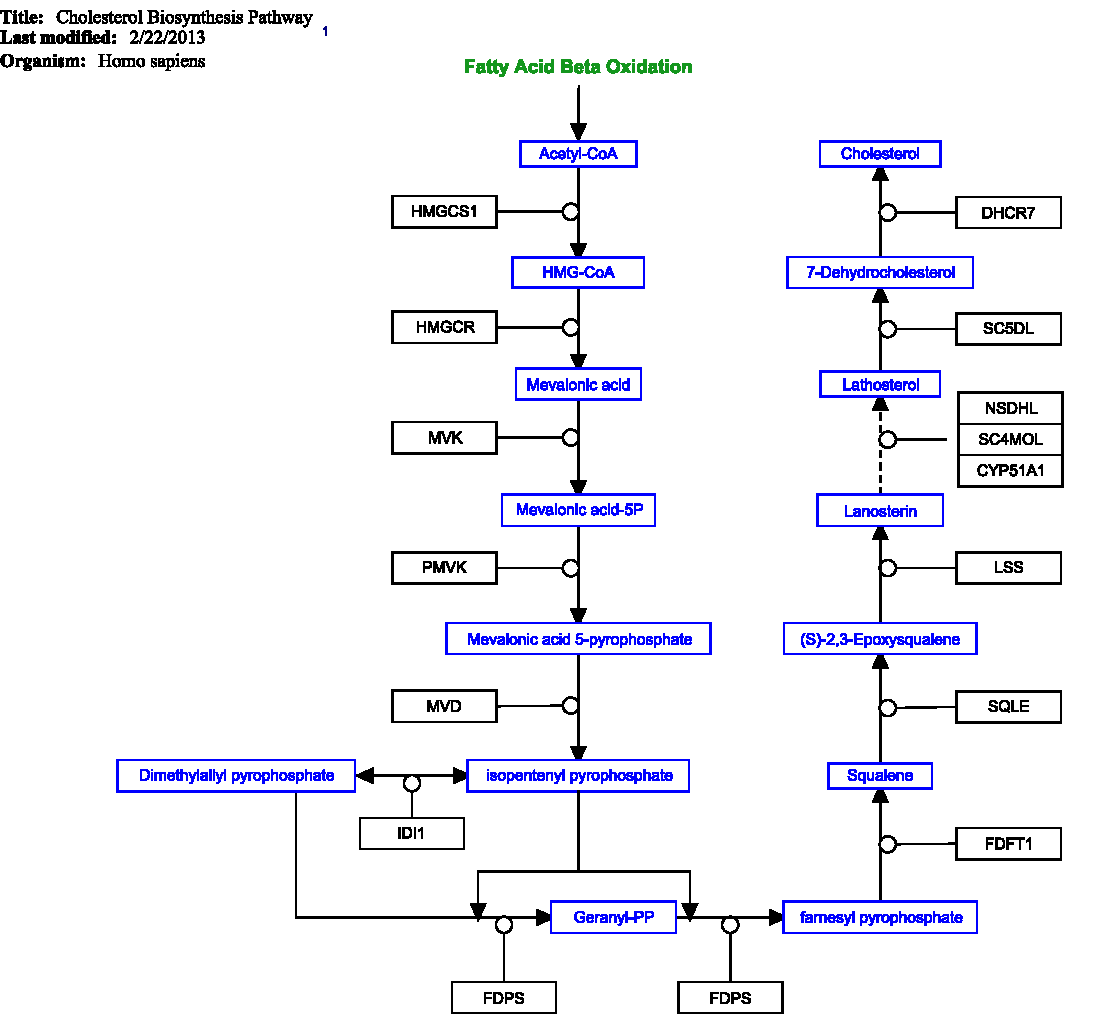
\includegraphics[width = 1.0 \textwidth ]{./Results/path4.pdf}
	\caption{\lr{Cholesterol Biosynthesis Pathway}}
	\label{fig:heat}
\end{figure}


\newpage

\subsubsection{تحلیل\lr{ Gene Ontology}}

در مورد \lr{Gene Ontology} ، اصلی‌ترین موردی که با \lr{APV} پایین دیده می‌شود مربوط به دو \lr{Cellular Component} با نام‌های \lr{MutLalpha complex (GO:0032389)}	 با
$APV = 0.005508$
 و 
\lr{	integral component of lumenal side of endoplasmic reticulum membrane (GO:0071556)}
با $APV=0.03364$ است و در هر دو مورد مقاله‌هایی مرتبط با موضوع یافت می‌شود. \cite{carcin,methylation}

\begin{latin}
	\begin{itemize}
		\item  {MutLalpha complex (GO:0032389)} : $APV = 0.005508$
	\end{itemize}
\end{latin}




\section{توضیحات مختلف در مورد \lr{AML}}

\subsection{آشنایی با \lr{AML}}

\subsubsection{\lr{AML} چیست؟}
برای بررسی \lr{AML} ابتدا باید ببینیم که لوکمی چیست.

لوکمی \LTRfootnote{Leukemia} به سرطان‌هایی می‌گونید که در سلول‌هایی ایجاد می‌شود که در حالت معمول، قرار است به سلول‌های مختلف خونی تبدیل شوند، مثل سلول های مغز استخوان که وظیفه تولید سلول های خونی را دارند. در رایج ترین شکل، لوکمی در حالات اولیه سلول‌های سفید خون ایجاد می‌شود اما در بعضی موارد، در سلول‌های دیگری هم این مسئله ایجاد می‌شود. لوکمی بسته به سرعت رشد به دو دسته  کلی حاد \LTRfootnote{Acute} یا مزمن 
\LTRfootnote{Chronic}
تقسیم می‌شوند. همچنین بعضی لوکمی‌ها در سلول‌های مربوط به مغزاستخوان
\LTRfootnote{myeloid}
شروع شده و برخی دیگر در سلول‌های لنفاوی
\LTRfootnote{lymphoid}
مانند غدد لنفاوی بدن ما.


لوکمی حاد مغزاستخوان، در بافت مغر استخوان -که قسمت نرم درونی برخی استخوان‌هاست که عموما این استخوان ها استخوان های بزرگی هستند و سلول‌های خونی در آن جا ساخته می‌شود- آغاز می‌شود. این نوع لوکمی در اغلب اوقات به سرعت به خون هم منتقل می‌شود. در حالت های حادتر، این لوکمی می‌تواند به بخش‌های دیگر بدن نظیر گره‌های لنفاوی، کبد،‌سیستم عصبی مرکزی (مغز و نخاع) و طحال هم متااستاتیز 
\LTRfootnote{metastasis}
بدهد و به آن‌ها گسترش یابد.





\subsubsection{مغز استخوان}

برای مطالعه بهتر این موضوع، باید بررسی کنیم که مغزاستخوان دقیقا چیست و چه وظیفه‌ای دارد.

مغز استخوان قسمت نرم درونی بعضی از استخوان‌های بدن است که عموما استخوان های درشت و بزرگی هستند و در سلول‌های تولید کننده خون، سلول‌های چربی و بافت همبند تشکیل شده است. بخش اندکی از سلول‌های تولید کننده خون، سلول‌های بنیادی خونی
\LTRfootnote{Blood Stem Cells}
 نامیده می‌شوند که این سلول های بنیادی خون میتوانند سلول های خونی دیگر را بوجود بیاورند.

درون مغز استخوان، این سلول‌های بنیادی خونی، به سلول‌های خونی مختلف تبدیل می‌شوند.  در طی این فرايند سلول‌های بنیادی خونی، یا تبدیل به لفنوسیت‌ها -که نوعی سلول سفید خونی است- تبدیل شده و یا به نوع دیگری از سلول‌های تولید کننده خون به نام میلوئید تبدیل می‌شوند. سلول‌های میلوئید می‌توانند تبدیل به گلبول‌های قرمز تبدیل شوند که امکان انتقال اکسیژن به نقاط مختلف بدن را دارند، یا به گلبول‌های سفید (متفاوت با لنفوسیت) که نقش ایجاد ایمنی بدن را دارند و یا به پلاکت تبدیل بشوند که ولاکت ها نقش انعقاد خون در هنگام پاره شدن رگ هارا دارند.  سلول‌هایی که در بیماری AML رفتار غیرنرمال دارند، همین سلول‌های میلوئید هستند.

\subsubsection{انواع سلول‌های خونی}

برای اطلاع بیش‌تر لازم است کمی در مورد سلول‌های خونی هم آگاهی پیدا کنیم.

به طور کلی سه نوع سلول اصلی خونی وجود دارد:

\begin{itemize}
	\item 
	 سلول‌های خونی قرمز: این سلول‌های وظیفه دارند که اکسیژن را از شش‌ها به همه بافت‌های مختلف بدن انتقال داده و در کربن دی‌اکسید تولیدی آن‌ها را به شش‌ها بازگردانند، در کلاس درس دکتر شریفی به ما پروتئینی را نشان دادند که امکان حمل اکسیژن را داشت و گفتند که آن پروتئین در گلبول های قرمز قرار دارند، شایان ذکر است گلبول های قرمز بالغ حاوی ماده ژنتیکی یا 
	 \lr{DNA}
	 نمیباشند و امکان تکثیر را به خودی خود ندارند.
	
	\item پلاکت‌ها: پلاکت‌ها در اصل قطعات سلولی هستند که توسط نوع خاصی از سلول‌های مغز استخوان موسوم به مگاکاریوسیت 
	\LTRfootnote{megakaryocyte}
	ساخته می‌شوند. یکی از اصلی‌ترین وظیفه پلاکت‌ها انعقاد خون در هنگام خون ریزی و جلوگیری از از دست دادن خون است. آن‌ها کمک می‌کنند سوراخ‌هایی که روی رگ‌ها در اثر ضربه یا خراش ایجاد شده است، پوشیده و مسدود شوند تا این بافت ها ترمیم شوند و خون زیاد از دست نرود، اگر مشکلی برای پلاکت ها ایجاد شود یا کم باشند ممکن است در اثر ساده ترین خراش ها خون زیادی از دست رود و زنده نمانیم!
	
	\item 
سلول‌های سفید خونی: وظیفه این سلول‌ها مبارزه با عفونت‌ها در بدن است که این کار را به روش های گوناگونی انجام میدهند، مثلا بلعیدن سلول مهاجم یا سرطانی یا تولید آنتی بادی و یا...
\end{itemize}

سلول‌های سفید، خود دسته‌های مختلفی دارند. از جمله مهم‌ترین آن‌ها سه دسته زیر است:

\begin{itemize}
	\item \lr{Granulocytes}: گرانولوسیت‌ها سلول‌های سفید بالغی هستند که از میلوبلاست‌‌ها 
	\LTRfootnote{Myeloblasts}
	که خود یک نوع سلول تولید کننده خون در مغز استخوان است، ایجاد می شود. گرانولوسیت‌ها به صورت سلول‌هایی که یکسری نقطه روی خود دارند زیر میکروسکوپ دیده می‌شوند. این نقاط شامل آنزیم‌ها و موادی هستند که می‌توااند میکروب‌‌ها را نابود کنند. سه نوع گرانولوسیت به نام‌های \lr{Neutrophil}، \lr{Basophil} و \lr{Eosinophil} وجود دارند.
	
	
	\item \lr{Monocytes}: مونوسیت‌ها از مونوبلاست‌ها
	\LTRfootnote{monoblasts}
	در مغز استخوان ایجاد می‌شوند. این سلول‌ها بعد از چرخیدن در سراسر بدن در طول حدود یک روز،‌ وارد بافت‌ها شده و تبدیل به ماکروفاژ
	\LTRfootnote{Macrophage}
	می‌شود. ماکروفاژ‌ها با احاطه کردن میکروب‌ها و هضم کردن‌ آنان به ایمنی بدن کمک کنند. این سلول‌ها به لنفوسیت‌ها در شناسایی میکروب‌ها و ترشح آنتی بادی مناسب هم کمک می کنند.
	
	\item \lr{Lymphocytes}: لنفوسیت‌ها، از لنفوبلاست
	\LTRfootnote{Lymphoblast}
	در مغز استخوان ایجاد می‌شوند. این سلول‌ها جزء اصلی سازنده بافت لنفاوی هستند که بخش بزرگی از سیستم ایمنی بدن است. بافت لنفاوی در گره‌های لنفاوی، تیموس، طحال و بخش‌های مختلفی از بدن یافت می‌شود. دو نوع اصلی لنفوسیت‌ها سلول‌های \lr{T} و \lr{B} نامیده می‌شوند.
\end{itemize}

 
 
 \subsubsection{ریسک فاکتور‌ها}
 
 عوامل مختلفی وجود دارند که می‌توانند باعث افزایش احتمال ابتلا به \lr{AML} بشوند. در زیر به طور خلاصه بعضی از این عوامل را ذکر کرده‌ایم:
 
 \begin{itemize}
 	\item 
سن: احتمال ابتلا با افزایش سن رابطه مستقیم دارد.
 	
 	\item
جنسیت : \lr{AML} در مردان شایع‌تر از زنان است.
 	
 	
 	\item
 سیگار کشیدن: همانند بسیاری از بیماری‌های دیگر، سیگار کشیدن احتمال ابتلا به \lr{AML} را هم افزایش می‌دهد. دلیل این موضوع این است که مواد سرطان زایی مانند نیکوتین و ... در مواد مخدر وجود دارد که در شش جذب شده و به سراسر بدن منتقل می ‌شوند و می‌توانند باعث ایجاد سرطان‌های مختلف بشوند.
 	
 	
 	\item
 	قرار گرفتن در معرض بعضی مواد شیمیایی: به عنوان مثال برخورد طولانی مدت با بنزن و فرمالدهید  (مثلا در محل کار) ریسک ابتلا به \lr{AML} را افزایش می‌دهند.
 	
 	\item 
قرار گرفتن در معرض مواد رادیواکتیو: همانند اکثر سرطان‌ها، قرار گرفتن در معرض پرتو‌های ناشی از مواد رادیواکتیو احتمال ابتدا به \lr{AML} را افزایش می‌دهد چراکه اشعه های ایکس و آلفا و بتا از این مواد ساتع میشوند که این توانایی را دارند تا به ماده ژنتیکی ا آسیب بزنند و موجب سرظان شوند یا سلول سرطانی را ایجاد کنند.
 	
 	
 	\item
 وجود یکسری ناهنجاری‌های خونی: بعضی از ناهنجاری‌ّای خونی نظیر \lr{myelodysplastic syndrome} احتمال ابتلا به \lr{AML} را بالا می‌برند. 
 	
 	
 	\item
 وجود مشکلات ژنتیکی: بعضی جهش‌های ژنتیکی نظیر \lr{Fancone Anemia} یا سندروم \lr{Bloom} یا مشکلات ژنتیکی خیلی شدیدتر نظیر مشکلات کروموزومی نظیر سندروم داون امکان ابتلا به \lr{AML} را افزایش می‌دهد.
 	
 	\item
 سابقه خانوادگی: افرادی که در خانواده خود افرادی با AML را داشته‌اند، احتمال ابتلا به این بیماری در آن‌ها بیش‌تر است. این همان عامل ژنتیکی است.
 	
 	

 \end{itemize}


\subsubsection{علائم \lr{AML}}
برای شناسایی زودهنگام این بیماری باید علائم آن را شناخت. علائم این بیماری را می‌توان به چند دسته تقسیم کرد.


\textbf{علائم ناشی از کمبود سلول‌های قرمز خونی:}

این علائم به دلیل کمبود سلول‌های قرمز خون پیش‌ می‌آیند. کمبول سلول‌های قرمز (کم خونی) می‌تواند به دلایل دیگری هم پیش بیاید ولی یکی از علل آن ممکن است \lr{AML} باشد. این علائم شامل موارد زیر است:

\begin{itemize}
	\item خستگی
	
	\item ضعف
	
	\item احساس سرما
	
	\item سرگیجه
	
	\item سردرد
	
	\item رنگ پریدگی
	
	\item تنگی نفس
	
\end{itemize}


\textbf{علائم ناشی از کمبود سلول‌های سفید نرمال خونی:}

سلول‌های سفید خونی مسئول مبارزه با عفونت‌ها و بیماری‌ها هستند. فرد مبتلا به \lr{AML} ممکن است به طور مداوم دچار بیماری‌های عفونی بشود که به راحتی برطرف نمی‌شوند و یا با فاصله کم بعد از بهبودی از یک بیماری، درگیری بعدی بشود.  با وجود این که در بیماران AML ممکن است تعداد سلول‌های سفید خون زیاد باشد، اما این افزایش تعداد به دلیل سلول‌های لوکمی هستند که از حالت رفتاری نرمال خارج شده و در مقابل بیماری‌های عفونی، از بدن محافظت نمی‌کنند.

\textbf{علائم ناشی از کمبود پلاکت}

این علائم شامل موارد زیر هستند:

\begin{itemize}
	\item کبودی‌های مختلف روی پوست
	
	
	\item خونریزی طولانی که بند نیاید
	
	\item خونریزی‌های شدید و متدوال بینی
	
	\item خونریزی لثه
	
	
\end{itemize}


\textbf{علائم ناشی از افزایش سلول‌های لوکمی}

سلول‌هیا سرطانی \lr{AML} معمولا بزرگ‌تر از سلول‌های معمول سفید خونی هستند و به آسانی نمی‌توانند در رگ‌ها جا به جا شوند. با این وجود اگر تعداد آن‌ها خیلی زیاد بشود، امکان ایجاد لخته‌های خونی درون رگ‌ها وجود دارد و در نتیجه آن سلول‌های قرمز هم امکان جا به جایی نخواهند داشت. به این پدیده Leukostasis گفته می‌شود. این پدیده نادر است ولی در صورت وقوع، باید به طور اورژانسی به آن رسیدگی شود. از علائم آن موارد زیر هستند:

\begin{itemize}
	\item سردرد
	
	\item ضعف در یک سمت بدن
	
	\item تکلم گنگ و نامفهوم
	
	\item گیجی و پریشانی
	
	\item خواب‌آلودگی
\end{itemize}



\textbf{علائم عمومی:}

علائم زیر علائم عمومی هستند که هر چند در \lr{AML} هم مشاهده می‌شوند اما در بسیاری از بیماری‌های دیگر هم وجود دارند و وجود آن‌ها به تنهایی احتمالا علت دیگری دارد.

\begin{itemize}
	\item کاهش وزن
	
	\item خستگی
	
	\item تب
	
	\item عرق شبانه
	
	\item کاهش اشتها
\end{itemize}

\textbf{علائم مربوط به پخش شدن بیماری به سایر اندام‌ها:}

در صورت انتشار لوکمی به سایر اندام‌های بدن و به خصوص انتقال به مغز و نخاع، علائم زیر ممکن است رخ بدهد:

\begin{itemize}
	\item سردرد
	
	\item ضعف
	
	\item حمله صرع
	
	\item استفراغ
	
	\item مشکل در تعادل
	
	\item بی حسی صورت
	
	\item تاری دید
	
\end{itemize}
\subsubsection{علت ابتلا به \lr{AML}}

پیدا کردن دلیل اصلی ابتدا به این بیماری در اکثر افراد کار دشواری است. با این وجود به طور کلی می‌توان در مورد علل ابتلا به این نوع سرطان توضیحاتی ارائه داد.

ژن‌های خاصی در سلول‌ها وجود دارند که مسئول رشد و تکثیر و مرگ سلول‌ها هستند. ژن‌هایی که مسئول رشد و تکثیر و زنده ماندن سلول هستند \lr{Oncogene} و سلول‌هایی که مسئول مرگ سلول در زمان مناسب هستند، ژن‌های سرکوب‌گر تومور
\LTRfootnote{Tumor Suppressor Gene}
نامیده می‌شوند.

از آن جایی که فرآیند تقسیم سلولی،  فرآیند کاملا دقیقی نیست و امکان خطا در آن وجود دارد، گاهی به دلیل جهش‌هایی خاص، \lr{Oncogene} ها بیش‌از حد انتظار فعال شده و یا ژن‌های سرکوب‌گر تومور، غیرفعال شوند. در چنین شراطی سلول به طور بی‌رویه به رشد و تکثیر ادامه داده و در تومور و در موارد شدیدتر سرطان ایجاد می شود. به طور مثلا در \lr{AML}، دیده شده که ژن‌هایی نظیر \lr{FLT3} یا \lr{RAS} در این زمینه نقش مهمی دارند.


تغییرات مختلفی ممکن است در کروموزوم‌های یک سلول AML اتفاق افتاده باشد که در درس به آنها پرداخته شد. بعضی از آن‌ها به شرح زیر است:

\begin{itemize}
	
	\item جا به جایی کروموزمی
	\LTRfootnote{Translocation}: این موضوع، شایع‌ترین مورد در تغییرات کروموزومی است. در این حالت بخشی از یک کروموزوم شکسته شده و به کروموزوم دیگر متصل می‌شود. در صورتی که این تغییر منجبر به فعال شدن Oncogene ها و یا غیرفعال شدن ژن‌های سرکوب کننده تومور نظیر \lr{RUNX1} بشود، امکان ایجاد تومور وجود دارد.
	
	\item حذف کروموزومی
	\LTRfootnote{Deletion}:
	در این حالت قسمتی از کروموژوم حذف می‌شود. این حذف ممکن است منجر به از دست رفتن ژن‌های سرکوب‌گر تومور بشود و در نتیجه رشد آن سلول  از کنترل خارج بشود.
	
	
	\item معکوس شدن
	\LTRfootnote{Inversion}:
	در این حالت، کروموژم معکوس شده و ترتیب آن برعکس می‌شود. در این حالت تعداد زیادی از ژن‌ها ممکن است از دست بروند. عملا این حالت مانند خواندن یک کتاب برعکس است. در نتیجه تعدادی زیادی از‌ ژن‌های مربوط به آن کروموزوم وظیفه خود را به درستی انجام نخواهند داد.
	
	
	\item تکرار
	\LTRfootnote{Addition or Duplication}: در این حالت، بخشی از کروموزوم تکرار می‌شود. این موضوع می‌تواند منجر به ایجاد کپی‌های زیادی از یک ژن درون سلول بشود و در نتیجه اگر این ژن‌ها جزو \lr{Oncogene} ها باشند، امکان تکثیر بی‌رویه سلول وجود دارد.
	
	  
	  
	
\end{itemize}


\subsubsection{پیشگیری از \lr{AML}}

با توجه به این که بسیاری از ریسک فاکتور‌های \lr{AML} موارد غیرقابل تغییر هستند، در اکثر موارد امکان جلوگیری از وقوع \lr{AML} در یک فرد وجود ندارد. با این حال، چندین عامل مهم وجود دارند که کنترل آن‌ها می‌تواند به پیشگیری از این سرطان منجر شود.

اولین مورد که اصلی ترین عامل قابل کنترل است، جلوگیری از سیگار کشیدن است. سیگار و دخانیات رابطه مستقیم با ابتلا به انواع سرطان‌ها دارند و کنترل این رفتار‌ها نیز کاملا بر عهده خود افراد است. در نتیجه جلوگیری از مصرف دخانیات نقش موثری در کاهش احتمال ابتلا به \lr{AML} دارد.

شیمی درمانی و قرار گرفتن در معرض تابش مواد رادیواکتیو، هر چند برای درمان یک سرطان دیگر استفاده می‌شود اما ممکن است باعث ایجاد نوع دیگر سرطان نظیر \lr{AML} بشود. در حال حاضر تحقیقات مختلفی در دنیا در حال انجام است تا روش‌هایی برای این کار پیدا شود که باعث افزایش احتمال ابتلا به یک سرطان جانبی نشوند. با این حال، همچنان درمان سرطان‌های مهلک به کمک شیمی درمانی و پرتودرمانی، اهمیت بالایی دارد. زیرا هر چند ممکن است این درمان‌ها در آینده منجر به سرطان دیگری بشوند، اما حداقل باعث می‌شوند که سرطان فعلی فرد تا حد خوبی کنترل بشود و در نهایت منجر به افزایش طول عمر می‌شوند.

در صورتی که فرد با مواد شیمی سرطان‌زا نظیر بنزن کار می‌کند، احتمال ابتلای او به سرطان‌های مختلف نظیر \lr{AML}‌ افزایش می‌یابد. عوض کردن شغل و یا برخورد کاملا محافظت شده با این مواد می‌تواند به کاهش احتمال ابتلا به \lr{AML} موثر باشد.
 	
مطالب این مقدمه برگرفته از \cite{acs} 
 بودند.


\subsection{بررسی ارتباطات نتایج تحلیل دادگان ریزآرایه و AML}


در قسمت Pathway یکی از مواردی که به آن اشاره کردیم
\lr{Microglia Pathogen Phagocytosis Pathway}
بود. یکی از مقالاتی که به این موضوع پرداخته،\cite{microglia}
است. Microglia یا میکروگلیا، در اصل سلول‌هایی کوچک و غیرعصبی هستند که ساختار حمایتی دستگاه عصبی مرکزی را تشکیل می‌دهند. این سلول‌ها از جمله اولین سلول‌هایی هستند که نسبت به عفونت‌های مغزی نظیر انسفالوپاتی واکنش نشان می‌دهند. یکی از ژن‌های که خیلی به \lr{AML} مرتبط است،‌ ژن \lr{RUNX1} است که با نام \lr{AML1} هم شناخته می‌شود. این‌ژن در مراحلی از ایجاد میکروژلیا در دوران جنینی تاثیر دارد و باعث تغییرات ساختاری و مورفولوژیکی در آن می‌شود. افزایش آن در \lr{AML} باعث ایجاد اختلال‌هایی در کار‌های بدن می‌شود.


موضوع دیگر مربوط به \lr{TYROBP Causal Network} می شود. TYROBP نوعی پروتئین تیروزین کیناز 
\LTRfootnote{Tyrosine Kinase}
است. این پروتئین در تشکیل سلول‌های ایمنی (ایمونوگلوبین)‌ بدن نقش دارد و همان طور که می‌دانیم، در جریان \lr{AML} سلول‌های سفید خونی که فعالیت نرمالی ندارند، افزایش می‌یابند. در نتیجه رابطه بین این مورد با \lr{AML} هم مشخص می شود. 

این مورد در \cite{wikipedia2020}
  و  \cite{trombly}
   بررسی شده است.
   
   
   از طرف دیگر در بخش \lr{Gene Ontology}،  قسمت \lr{Biological Process} شاهد حضور مواردی مرتبط با \lr{Neutrophil} ها هستیم. همان طور که در بخش آشنایی با \lr{AML} گفته شد، \lr{Neutrophil} ها یکی از انواع گرانولوسیت‌ها هستند و گرانولوسیت‌ها خود جزو گلبول‌های سفید به حساب می‌آمدن. افزایش بیان ژن‌هایی که منجر به فعال‌سازی این سلول‌ها می‌شود با توجه به ذات \lr{AML} که منجر به تکثیر بی‌رویه سلول‌های خونی می‌شود، منطقی به نظر می‌رسد. در مقاله‌های \cite{lamble} و \cite{rosenblum} هم به افزایش فعالیت‌های مربوط به \lr{Neutrophil}‌ ها در \lr{AML} پرداخته شده است.
   
   
   در قسمت \lr{Molecular Function} مشاهده می کنیم که یکی از مواردی که وجود دارد \lr{Kinase Binding} است. کیناز یک آنزیم است که بر روی فسفات‌های پرانرژی نظیر \lr{ATP} اثر گذار است. در این بیماری شاهد این هستیم که ژن‌هایی مربوط به فرآیندهای \lr{Kinase} بیان ‌بیش‌تری داشته‌اند. با تحقیق در مقالات، می‌بینیم که این مسئله به شکل خیلی جدی بررسی شده است. یکی از درمان‌هایی که برای \lr{AML} پیشنهاد می‌شود، مبتنی بر استفاده از بازدارنده‌های تیروزین کیناز
   \LTRfootnote{Tyrosine Kinase Inhibitor}
   و بازدارنده‌های ترئونین/سرین کیناز
   \LTRfootnote{Serine/Threonine Kinase inhibitors}
   است. مکانیزم اثر این داروها به این شکل است که در برای پیوند دادن با کیناز، با \lr{ATP} وارد رقابت شده و سعی می‌کنند در مواردی باعث ‌شوند که \lr{ATP} نتواند با کیناز وارد پیوند کاتالیزی بشود. در نتیجه بدین شکل جلوی فعالیت بیش از حد کیناز را می‌گیرند. از این دارو‌ها در سرطان‌های دیگر هم استفاده می‌شود. مقاله \cite{HARI2014628} به این دارو‌ها پرداخته و مقاله \cite{kinase} هم به بررسی تاثیر این دارو‌ها در \lr{AML} و پیشرفت‌ها و چالش‌های پیش‌رو در استفاده از آنان پرداخته است.
   
   
 
   در مورد \lr{Gene Ontology} های مربوط به کاهش بیان ژن، به \lr{MutLAlpha} اشاره شد. در اصل \lr{MutL} ها جزو سیستم اصلاح اشتباهات \lr{DNA} 
   \LTRfootnote{DNA Mismatch Repair}
    هستند. این که مشاهده‌ می‌کنیم در هنگام وقوع این سرطان، بیان ژن‌های مربوط به آن کاهش یافته است، امری منطقی است. زیرا عملا این سرطان و ایجاد سلول‌هایی که رشد‌ آن‌ها به صورت بی‌رویه است، همان طور که در بخش‌های قبل هم گفتیم در اثر ایرادات و اشتباهاتی که در تقسیم سلولی روی می‌دهد اتفاق می‌افتد که ژن‌های نامناسبی فعال می‌شوند. در این مورد سیستم اصلاح اشتباهات دچار مشکل شده و در نتیجه آن این سلول‌های نامعمول لوکمی ایجاد شده‌اند. این موضوع در \cite{carcin} بررسی شده است.
    
    \section{بررسی روش های دیگر کاهش ابعاد}
برای کاهش ابعاد، سه دسته روش کلی داریم:
\begin{itemize}
	
	\item 
	روش هایی که ویژگی های متنوعی را نگه میدارند که شامل روش های خطی و روش های غیر خطی میشود.
	
	\item 	  
	  روش هایی که فقط مهم ترین ویژگی هارا نگه میدارند
\end{itemize}

  \subsection{روش های خطی}
  این روش ها شامل موارد زیر هستند:
  
   \begin{itemize}
	
	\item 
	\lr{PCA}
: 
\lr{PCA}
 یکی از الگوریتم های یادگیری ماشینی مورد علاقه من است. \lr{PCA} یک تکنیک کاهش ابعاد خطی (الگوریتم) است که مجموعه‌ای از متغیرهای همبسته (\lr{p}) را به تعداد \lr{k}
  (\lr{k}<\lr{p})
  کوچکتر از متغیرهای غیرهمبسته به نام مؤلفه‌های اصلی تبدیل می‌کند و در عین حال تا آنجا که ممکن است تغییرات در مجموعه داده اصلی را حفظ می‌کند. در زمینه یادگیری ماشینی (\lr{ML})، \lr{PCA} یک الگوریتم یادگیری ماشینی بدون نظارت است که برای کاهش ابعاد استفاده می شود و این روش همان روش مورد استفاده ما بود.
  
	\item 	
	\lr{FA}
	:
تحلیل عاملی (\lr{FA}) و تجزیه و تحلیل مؤلفه اصلی (\lr{PCA}) هر دو تکنیک کاهش ابعاد هستند. هدف اصلی تحلیل عاملی فقط کاهش ابعاد داده ها نیست. تحلیل عاملی یک رویکرد مفید برای یافتن متغیرهای پنهانی است که مستقیماً در یک متغیر اندازه‌گیری نمی‌شوند، بلکه از سایر متغیرهای مجموعه داده استنتاج می‌شوند. به این متغیرهای پنهان، عوامل می گویند.
	\item
	\lr{LDA}
	:
\lr{LDA}
 معمولاً برای طبقه بندی چند طبقه استفاده می شود. همچنین می توان از آن به عنوان تکنیک کاهش ابعاد استفاده کرد. \lr{LDA} به بهترین وجه نمونه‌های آموزشی را بر اساس کلاس‌هایشان جدا یا متمایز می‌کند (از این رو \lr{LDA} نامیده می‌شود). تفاوت عمده بین \lr{LDA} و \lr{PCA} در این است که \lr{LDA} ترکیبی خطی از ویژگی‌های ورودی را پیدا می‌کند که تفکیک‌پذیری کلاس‌ها را بهینه می‌کند در حالی که \lr{\lr{LDA}} تلاش می‌کند مجموعه‌ای از اجزای نامرتبط حداکثر واریانس را در یک مجموعه داده پیدا کند. تفاوت اصلی دیگر بین این دو این است که PCA یک الگوریتم بدون نظارت است در حالی که \lr{LDA} یک الگوریتم نظارت شده است که در آن برچسب های کلاس را در نظر می گیرد. \lr{LDA} محدودیت هایی دارد. برای اعمال \lr{LDA}، داده ها باید به طور معمول توزیع شوند. مجموعه داده همچنین باید حاوی برچسب های کلاس شناخته شده باشد. حداکثر تعداد مؤلفه هایی که \lr{LDA} می تواند پیدا کند، تعداد کلاس ها منهای \lr{1} است. اگر فقط \lr{3} برچسب کلاس در مجموعه داده شما وجود داشته باشد، \lr{LDA} می تواند تنها \lr{2} مؤلفه (\lr{3}–\lr{1}) را در کاهش ابعاد پیدا کند. برای اعمال \lr{LDA} نیازی به مقیاس بندی ویژگی نیست. از طرف دیگر، \lr{PCA} به داده های مقیاس شده نیاز دارد. با این حال، برچسب های کلاس برای \lr{PCA} مورد نیاز نیست. حداکثر تعداد مؤلفه‌هایی که \lr{PCA} می‌تواند پیدا کند، تعداد ویژگی‌های ورودی در مجموعه داده اصلی است.
	
	\item  
	\lr{Truncated SVD}
	:
این روش کاهش ابعاد خطی را با استفاده از تجزیه مقدار منفرد کوتاه (\lr{SVD}) انجام می دهد. با داده های پراکنده که در آن بسیاری از مقادیر ردیف صفر هستند، به خوبی کار می کند. در مقابل، \lr{PCA} با داده های متراکم به خوبی کار می کند. \lr{SVD} کوتاه شده همچنین می تواند با داده های متراکم استفاده شود. تفاوت اصلی دیگر بین \lr{SVD} کوتاه شده و \lr{PCA} این است که فاکتورسازی برای \lr{SVD} روی ماتریس داده انجام می شود در حالی که فاکتورسازی برای \lr{PCA} روی ماتریس کوواریانس انجام می شود.

\end{itemize}

  \subsection{روش های غیر خطی}

\begin{itemize}
	
	\item 
	\lr{Kernel PCA}
	:
	هسته \lr{PCA} یک تکنیک کاهش ابعاد غیر خطی است که از هسته ها استفاده می کند. همچنین می توان آن را به عنوان شکل غیر خطی \lr{PCA} معمولی در نظر گرفت. هسته \lr{PCA} با مجموعه داده های غیر خطی که در آن \lr{PCA} معمولی نمی تواند به طور موثر استفاده شود، به خوبی کار می کند.
شهود پشت هسته \lr{PCA} چیز جالبی است. داده ها ابتدا از طریق یک تابع هسته اجرا می شوند و به طور موقت آنها را به یک فضای ویژگی با ابعاد بالاتر جدید می فرستند، جایی که کلاس ها به صورت خطی قابل تفکیک می شوند (کلاس ها را می توان با کشیدن یک خط مستقیم تقسیم کرد). سپس الگوریتم از \lr{PCA} معمولی استفاده می‌کند تا داده‌ها را به فضایی با ابعاد پایین‌تر بازتاب دهد. به این ترتیب، هسته \lr{PCA} داده‌های غیرخطی را به فضایی با ابعاد پایین‌تر از داده‌ها تبدیل می‌کند که می‌تواند با طبقه‌بندی‌کننده‌های خطی استفاده شود.
	
	\item 
	\lr{t-SNE}
	:
	این نیز یک روش کاهش ابعاد غیر خطی است که بیشتر برای تجسم داده ها استفاده می شود. علاوه بر آن، به طور گسترده ای در پردازش تصویر و \lr{NLP} استفاده می شود. اسناد \lr{Sci-kit learn} به شما توصیه می‌کنند که از \lr{PCA} یا \lr{Truncated SVD} قبل از \lr{t-SNE} استفاده کنید، اگر تعداد ویژگی‌های مجموعه داده بیش از \lr{50} باشد. در زیر دستور کلی برای انجام \lr{t-SNE} بعد از \lr{PCA} آمده است. همچنین، توجه داشته باشید که قبل از \lr{PCA}، مقیاس‌بندی ویژگی لازم است.
	\item 
	\lr{MDS}
	:
	 یکی دیگر از تکنیک‌های کاهش ابعاد غیرخطی است که سعی می‌کند فاصله بین نمونه‌ها را حفظ کند و در عین حال ابعاد داده‌های غیرخطی را کاهش دهد. دو نوع الگوریتم \lr{MDS} وجود دارد: متریک و غیر متریک. کلاس \lr{MDS} در \lr{Scikit-learn} هر دو را با تنظیم هایپرپارامتر متریک روی \lr{True} (برای نوع متریک) یا \lr{False} (برای نوع غیر متریک) اجرا می کند.
	\item 
	\lr{Isomap}
	:
	این روش کاهش ابعاد غیر خطی را از طریق نقشه برداری ایزومتریک انجام می دهد. این افزونه \lr{MDS} یا \lr{Kernel PCA} است. هر نمونه را با محاسبه فاصله منحنی یا ژئودزیکی به نزدیکترین همسایگانش متصل می کند و ابعاد را کاهش می دهد. تعداد همسایگانی که برای هر نقطه باید در نظر گرفته شود را می توان از طریق هایپرپارامتر \lr{n-neighbors} کلاس \lr{Isomap} که الگوریتم \lr{Isomap} را در \lr{Scikit-learn} پیاده سازی می کند، مشخص کرد.
\end{itemize}

  \subsection{روش هایی که فقط مهم ترین ویژگی هارا نگه میدارند}
\begin{itemize}
	
	\item 
	\lr{Backward-elimination}:
	این روش ویژگی ها را از یک مجموعه داده از طریق فرآیند حذف ویژگی بازگشتی (\lr{RFE}) حذف می کند (حذف می کند). الگوریتم ابتدا سعی می کند مدل را بر روی مجموعه اولیه ویژگی ها در مجموعه داده آموزش دهد و عملکرد مدل را محاسبه می کند (معمولاً امتیاز دقت برای یک مدل طبقه بندی و \lr{RMSE} برای یک مدل رگرسیون). سپس، الگوریتم هر بار یک ویژگی (متغیر) را حذف می کند، مدل را بر روی ویژگی های باقی مانده آموزش می دهد و امتیازات عملکرد را محاسبه می کند. الگوریتم حذف ویژگی ها را تکرار می کند تا زمانی که یک تغییر کوچک (یا بدون) در امتیاز عملکرد مدل تشخیص دهد و در آنجا متوقف شود.
	\item 
	\lr{Forward selection}:
	این روش را می‌توان به‌عنوان فرآیند معکوس حذف معکوس در نظر گرفت. به جای حذف بازگشتی ویژگی ها، الگوریتم سعی می کند مدل را بر روی یک ویژگی واحد در مجموعه داده آموزش دهد و عملکرد مدل را محاسبه می کند (معمولاً امتیاز دقت برای مدل طبقه بندی و \lr{RMSE} برای مدل رگرسیون). سپس، الگوریتم هر بار یک ویژگی (متغیر) را اضافه می کند (انتخاب می کند)، مدل را بر روی آن ویژگی ها آموزش می دهد و امتیازات عملکرد را محاسبه می کند. الگوریتم اضافه کردن ویژگی ها را تکرار می کند تا زمانی که یک تغییر کوچک (یا بدون) در امتیاز عملکرد مدل تشخیص دهد و در آنجا متوقف شود!
	\item 
	\lr{Random forests}:
	جنگل های تصادفی یک مدل مبتنی بر درخت است که به طور گسترده برای کارهای رگرسیون و طبقه بندی بر روی داده های غیر خطی استفاده می شود. همچنین می‌توان از آن برای انتخاب ویژگی با ویژگی \lr{feature importances} داخلی خود استفاده کرد که امتیازات اهمیت ویژگی را برای هر ویژگی بر اساس معیار "\lr{gini}`` (معیار کیفیت تقسیم گره‌های داخلی) در حین آموزش مدل محاسبه می‌کند.
	
\end{itemize}
در نهایت به نظر می آید تمامی این روش ها کاری که ما نیاز داریم را انجام میدهند، روش PCA بسیار ساده است و بسیار گویا، بنابراین از این روش استفاده کردیم اما تمامی این روش ها میتوانستند مورد استفاده ما قرار بگیرند.

    
   \section{فایل‌های تحویلی}
   در پوشه \lr{Sourse}  فایل \lr{main.r}  قرار دارد که سورس اصلی کدها است، کل کد های این پروژه را با دیدن ویدیو های دکتر شریفی نوشتم و آنالیز هارا هم  به همان روش گفته شده انجام دادم، در کد سعی کردم برای هر تکه‌ای کامنت مناسب قرار دهم تا مشخص باشد چه کاری انجام میدهم.
   
   در پوشه \lr{Results} نتایج بدست آمده نظیر نمودارها و همچنین فایل های \lr{txt} شامل اسامی ژ‌‌ن‌هایی که تفاوت بیان داشته‌اند و همچنین جدولی که بعد از فیت کردن مدل‌ نهایی بدست آمده، قرار گرفته است.
   
   در نهایت این فایل گزارش که در حال مطالعه آن هستید هم در کنار این فایل‌ها قرار گرفته است.
   

   \section{نتیجه‌گیری نهایی}
   
   در این پروژه، ما به تحلیل داده‌های ریزآرایه برای بیماری لوکمی حاد مغزاستخوان پرداختیم. ابتدا به تحلیل مواردی نظیر همبستگی نمونه‌های مختلف پرداخته و پس از آن با توجه به شباهت بین دسته‌ای از نمونه‌های بیمار با سلول‌های \lr{CD34}، اقدام به تحلیل تفاوت بیان ژن در آن‌ها کردیم. در نهایت براساس این تفاوت‌ها و به کمک \lr{Enirchr}، در مورد \lr{Pathway}‌ ها و \lr{Gene Ontology} های مربوط به آن اطلاعاتی کسب کردیم. در بخش‌هایی نهایی نیز توضیحاتی در مورد خود بیماری \lr{AML} داده و همچنین به بررسی نتایجی که در مقالات دیگر مرتبط با این بیماری و \lr{Pathway} و \lr{Gene Ontology} های مربوطه وجود دارد، پرداختیم.
   در انتها هم با ذکر چندین مقاله و دارو کمی توضیح راجع به بیماری و روش های درمان و روش های پیشگیری از آن و علائم آن دادم.
   
   
   
   


 \setLTRbibitems
\makeatletter
\bidi@AtBeginEnvironment{thebibliography}{\latinfont}
\makeatother
\bibliographystyle{unsrt}
\bibliography{sample}
\end{document}



